% !TeX program = xelatex
% English publication copy adapted from the 43-page handwritten transcription.
% Source pp. 35--40 supply the stage summary; the appendix occupies pp. 41--43.
% Approved domain correction on source p. 33: enlargement of the Haar domain gives an inequality.
% Approved local amendment: define Omega on source p. 16, retain the domain
% in the sector integral and use {z : m+gz in Omega} after the change of variables.
\documentclass[10pt,reqno]{amsart}
\usepackage[margin=1in]{geometry}
\usepackage{amsmath,amssymb,amsthm,mathtools,bm}
\usepackage{graphicx,xcolor,enumitem,indentfirst}
\usepackage[protrusion=true,expansion=false]{microtype}
\usepackage{needspace}
\usepackage[section]{placeins}
\setcounter{tocdepth}{1}
\theoremstyle{definition}
\newtheorem{definition}{Definition}[section]
\newtheorem{lemma}[definition]{Lemma}
\newtheorem{example}[definition]{Example}
\theoremstyle{remark}
\newtheorem{remark}[definition]{Remark}
\numberwithin{equation}{section}
\numberwithin{figure}{section}
\setlength{\textfloatsep}{12pt plus 3pt minus 2pt}
\setlength{\intextsep}{10pt plus 3pt minus 2pt}
\setlength{\abovecaptionskip}{5pt}
\renewcommand{\topfraction}{.85}
\renewcommand{\bottomfraction}{.7}
\renewcommand{\textfraction}{.12}
\AddToHook{cmd/section/before}{\Needspace{6\baselineskip}}
\AddToHook{cmd/subsection/before}{\Needspace{4\baselineskip}}
% All seven diagrams below are native, editable TikZ; no image files are used.
\usepackage{tikz}
\usetikzlibrary{arrows.meta,decorations.markings,decorations.pathreplacing}
\tikzset{
  ym/base/.style={font=\small, line cap=round, line join=round},
  ym/edge/.style={draw=black, line width=.8pt},
  ym/grid/.style={draw=black!35, line width=.45pt},
  ym/path/.style={draw=black, line width=1pt},
  ym/midarrow/.style={ym/edge,
    postaction={decorate},
    decoration={markings,mark=at position .55 with
      {\arrow{Stealth[length=4.2pt,width=3.4pt]}}}},
  ym/arrow/.style={ym/edge,-{Stealth[length=4.2pt,width=3.4pt]}},
  ym/brace/.style={draw=black,line width=.55pt,
    decorate,decoration={brace,mirror,amplitude=3pt}},
  ym/dot/.style={circle,fill=black,inner sep=1.15pt}
}

\usepackage{hyperref}
\setlength{\parindent}{2em}
\setlength{\parskip}{0pt}
\linespread{1.1}
\AtBeginDocument{%
  \setlength{\abovedisplayskip}{7pt plus 2pt minus 2pt}%
  \setlength{\belowdisplayskip}{7pt plus 2pt minus 2pt}%
  \setlength{\abovedisplayshortskip}{3pt plus 1pt}%
  \setlength{\belowdisplayshortskip}{5pt plus 2pt minus 1pt}}
\raggedbottom
\clubpenalty=10000
\widowpenalty=10000
\displaywidowpenalty=10000
\allowdisplaybreaks[1]
\setlist[enumerate]{leftmargin=2em,itemsep=3pt,topsep=3pt}
\newcommand{\g}{\mathfrak g}
\newcommand{\dd}{\mathrm d}
\newcommand{\id}{\mathrm{id}}
\newcommand{\YM}{\mathrm{YM}}
\newcommand{\R}{\mathbb R}
\newcommand{\C}{\mathbb C}
\newcommand{\Z}{\mathbb Z}
\newcommand{\e}{\varepsilon}
\newcommand{\Ia}{I_{\mathrm a}}
\newcommand{\If}{I_{\mathrm f}}
\newcommand{\Uf}{\mathcal U_{\mathrm f}}
\newcommand{\Uc}{\mathcal U_{\mathrm c}}
\newcommand{\Hf}{H_{\mathrm f}}
\newcommand{\Hc}{H_{\mathrm c}}
\newcommand{\Fc}{F_{\mathrm c}}
\newcommand{\Gc}{G_{\mathrm c}}
\newcommand{\Oc}{O_{\mathrm c}}
\newcommand{\muc}{\mu_{\mathrm c}}
\DeclareMathOperator{\Ad}{Ad}
\DeclareMathOperator{\ad}{ad}
\DeclareMathOperator{\tr}{tr}
\DeclareMathOperator{\Vol}{Vol}
\setlength{\emergencystretch}{2em}
\hypersetup{pdftitle={Lattice Yang--Mills: Wilson measure and exact blocking},pdfauthor={Zexi He}}
\title[Lattice Yang--Mills: study notes]{Lattice Yang--Mills:\\Wilson measure and exact blocking}
\author{Zexi He}
\date{}
\AddToHook{cmd/@setauthors/after}{%
  \begingroup\centering\normalfont\footnotesize
  Personal study notes --- 15 November 2026\par\endgroup}
\begin{document}

\maketitle
\begin{list}{}{\leftmargin=1em\rightmargin=1em\topsep=4pt\parsep=0pt}
\item[]\small
These notes were developed from my handwritten study notes and transcribed,
translated and edited with AI assistance. They accompany the AI-generated
working exposition \cite{Exposition}, based on the OpenAI Yang--Mills Lean
project; source provenance and review limits are described in the repository
README. This installment covers the Wilson measure, exact blocking, tree gauge,
exponential coordinates, the central Gaussian estimate, conditional tail
bounds and a summary of exact sector reassembly. The model-dependent inputs
are stated explicitly; the continuum
construction is not established here. Corrections and missing references are welcome.
\end{list}

\tableofcontents
\medskip

\section{The Wilson measure}\label{sec:wilson}
We first recall the Wilson action and the lattice Yang--Mills measure.
Let $G$ be a closed subgroup of $U(N)$, with Lie algebra $\g$. Write $h_G$ for normalized Haar measure and $e_i$ for the coordinate unit vectors. Set
\begin{equation}\label{eq:display-001}
\Lambda_\ell=(\Z/\ell\Z)^4,
\qquad
\mathcal U_\ell:=G^{\Lambda_\ell\times\{1,2,3,4\}}.
\end{equation}
The positively oriented edges are $E_\ell^+=\Lambda_\ell\times\{1,2,3,4\}$.

A configuration $U\in\mathcal U_\ell$ assigns $U(x,i)\in G$ to the oriented link from $x$ to $x+e_i$;
the reverse link carries $U(x,i)^{-1}$.

The product Haar measure on $\mathcal U_\ell$ is
\begin{equation}\label{eq:display-002}
H_\ell=\bigotimes_{(x,i)\in\Lambda_\ell\times\{1,2,3,4\}}h_G.
\end{equation}

\begin{definition}[Plaquette holonomy] For $1\le i<j\le4$, define the holonomy around the plaquette in Figure~\ref{fig:plaquette} by



\begin{equation}\label{eq:plaquette-holonomy}
P_{ij}(U;x)
 =U(x,i)U(x+e_i,j)U(x+e_j,i)^{-1}U(x,j)^{-1}.
\end{equation}
\end{definition}

\begin{figure}[htbp]
\centering
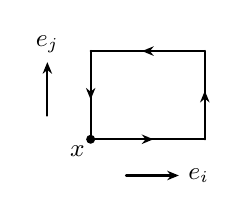
\begin{tikzpicture}[ym/base]
  \coordinate (x) at (0,0);
  \coordinate (xi) at (1.45,0);
  \coordinate (xij) at (1.45,1.12);
  \coordinate (xj) at (0,1.12);
  \draw[ym/midarrow] (x) -- (xi);
  \draw[ym/midarrow] (xi) -- (xij);
  \draw[ym/midarrow] (xij) -- (xj);
  \draw[ym/midarrow] (xj) -- (x);
  \node[ym/dot] at (x) {};
  \node[below left,inner sep=2pt] at (x) {$x$};
  \draw[ym/arrow] (.45,-.46) -- (1.12,-.46)
    node[right,inner sep=3pt] {$e_i$};
  \draw[ym/arrow] (-.55,.30) -- (-.55,.98)
    node[above,inner sep=3pt] {$e_j$};
\end{tikzpicture}
\caption{The positively oriented plaquette based at $x$.}
\label{fig:plaquette}
\end{figure}

\begin{definition}[Wilson measure]
The Wilson energy is
\begin{equation}\label{eq:wilson-energy}
W_\ell(U)=\sum_{x\in\Lambda_\ell}\sum_{i<j}
 \left(1-\frac1N\operatorname{Re}\tr P_{ij}(U;x)\right).
\end{equation}
For $\beta\in\R$, set
\begin{equation}\label{eq:partition-function}
Z_\ell(\beta):=\int_{\mathcal U_\ell}e^{-\beta W_\ell(U)}\,\dd H_\ell(U),
\end{equation}
\begin{equation}\label{eq:wilson-measure}
\dd\mu_{\ell,\beta}(U)
 =Z_\ell(\beta)^{-1}e^{-\beta W_\ell(U)}\,\dd H_\ell(U).
\end{equation}
\end{definition}

This convention makes the scaling factors explicit in subsequent renormalization-group calculations.

\begin{remark} Distances in $\Lambda_\ell$ are measured in lattice units; $\ell$ is the number of sites in each coordinate direction.
At mesh $\e$, the physical side length is $M=\e\ell$.
In four dimensions, no explicit power of $\e$ occurs in this definition of $\mu_{\ell,\beta}$.

\end{remark}

\subsection{Relation to the continuum action}
For this scaling calculation only, use the $d$-dimensional analogue $\Lambda_\ell=(\Z/\ell\Z)^d$. Consider, formally,
\begin{equation}\label{eq:display-007}
\Lambda_{M,\e}=(\e\Z/M\Z)^d,
\qquad
\mu^{\YM}(\dd A)\propto\exp\bigl(-S(A)\bigr)\,\dd A,
\end{equation}
\begin{equation}\label{eq:display-008}
S(A)=\int_{\R^d}|F_A|^2\,\dd x,
\qquad (F_A)_{ij}=[D_{A,i},D_{A,j}].
\end{equation}
Here $A$ is smooth, $D_{A,i}=\partial_i+A_i$, and the continuum curvature is the matrix coefficient of this commutator. The symbol $\dd A$ is formal; no infinite-dimensional Lebesgue measure is being defined.
The corresponding lattice expression is
\begin{equation}\label{eq:display-009}
\int_{\R^d}|F_A|^2\,\dd x
\leadsto
\e^d\sum_{x\in\Lambda_\ell}\sum_{i<j}
\operatorname{Re}\tr\bigl((F_U)_{ij}(F_U)_{ij}^*\bigr).
\end{equation}

For a lattice function $f$ with values in $\C^N$, define
\begin{equation}\label{eq:display-010}
(D_{U,i}f)(x):=\e^{-1}\bigl(U(x,i)f(x+e_i)-f(x)\bigr).
\end{equation}
Then
\begin{equation}\label{eq:display-011}
([D_{U,i},D_{U,j}]f)(x)
=(F_U)_{ij}(x)f(x+e_i+e_j).
\end{equation}
The matrix $(F_U)_{ij}(x)$ is the coefficient after extracting the common endpoint shift. The two paths are shown in Figure~\ref{fig:curvature}.

\begin{figure}[htbp]
\centering
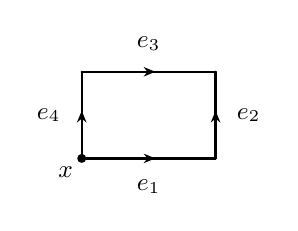
\begin{tikzpicture}[ym/base]
  \draw[ym/midarrow] (0,0) -- (1.70,0)
    node[midway,below=4pt] {$e_1$};
  \draw[ym/midarrow] (1.70,0) -- (1.70,1.10)
    node[midway,right=4pt] {$e_2$};
  \draw[ym/midarrow] (0,1.10) -- (1.70,1.10)
    node[midway,above=4pt] {$e_3$};
  \draw[ym/midarrow] (0,0) -- (0,1.10)
    node[midway,left=4pt] {$e_4$};
  \node[ym/dot] at (0,0) {};
  \node[below left,inner sep=3pt] at (0,0) {$x$};
\end{tikzpicture}
\caption{The two paths from $x$ to $x+e_i+e_j$; the top and left edges point right and up.}
\label{fig:curvature}
\end{figure}

\begin{equation}\label{eq:lattice-curvature}
(F_U)_{ij}(x)=\frac1{\e^2}\left(U_{e_1}U_{e_2}-U_{e_4}U_{e_3}\right).
\end{equation}
Thus
\begin{equation}\label{eq:display-013}
\e^d\sum_{x\in\Lambda_\ell}\sum_{i<j}
\operatorname{Re}\tr\bigl((F_U)_{ij}(F_U)_{ij}^*\bigr) =2\e^{d-4}\sum_{x\in\Lambda_\ell}\sum_{i<j}
\left(N-\operatorname{Re}\tr\bigl(P_{ij}(U;x)\bigr)\right).
\end{equation}
For $d=4$,
\begin{equation}\label{eq:display-014}
\mu_{M,\e}(\dd U)
\propto\exp\left(-C\sum_{x\in\Lambda_\ell}\sum_{i<j}
\left(N-\operatorname{Re}\tr\bigl(P_{ij}(U;x)\bigr)\right)\right) \times\dd H_{M,\e}(U).
\end{equation}
At fixed coupling, its dependence on $M,\e$ is through $\ell=M/\e$.

\begin{remark}[Normalization]
We write $C=\beta/N$. With $N$ fixed, this is a parametrization of the coupling; no large-$N$ limit is considered here.

\end{remark}

\begin{lemma}\label{lem:wilson-bound} $W_\ell$ is continuous and
\begin{equation}\label{eq:display-015}
0\le W_\ell(U)\le12\ell^4.
\end{equation}
\end{lemma}

\begin{proof}
\begin{equation}\label{eq:display-016}
W_\ell(U)=\sum_{x\in\Lambda_\ell}\sum_{i<j}
\left(1-\frac1N\operatorname{Re}\tr P_{ij}(U;x)\right).
\end{equation}
For $P\in U(N)$, each diagonal entry satisfies $|P_{aa}|\le1$.
Indeed,
\begin{equation}\label{eq:display-017}
PP^*=I\quad\Longrightarrow\quad
\sum_bP_{ab}\overline{P_{cb}}=\delta_{ac}
\quad\Longrightarrow\quad\sum_b|P_{ab}|^2=1.
\end{equation}
Hence
\begin{equation}\label{eq:display-018}
\bigl|\operatorname{Re}\tr P_{ij}(U;x)\bigr|\le N,
\end{equation}
so that
\begin{equation}\label{eq:display-019}
0\le W_\ell(U)\le\ell^4\binom42\times2=12\ell^4.
\end{equation}
\end{proof}

\subsection{Gauge invariance and observables}
For $t:\Lambda_\ell\to G$,
\begin{equation}\label{eq:display-020}
U^t(x,i)=t(x)U(x,i)t(x+e_i)^{-1}.
\end{equation}
Then
\begin{equation}\label{eq:display-021}
P_{ij}(U^t;x)=t(x)P_{ij}(U;x)t(x)^{-1},
\qquad W_\ell(U^t)=W_\ell(U).
\end{equation}
Introduce the lattice spacing $\e_n$ and physical side length $M$:
\begin{equation}\label{eq:display-022}
\e:=\e_n=\frac1n,
\qquad \ell:=\ell_{n,M}=M/\e_n.
\end{equation}
The eventual aim is to study the limits $n\to\infty$ and $M\to\infty$.

\begin{definition}[Local gauge-invariant observables]
Let $\mathcal V$ be a label set. A family of local gauge-invariant observables is written as
\begin{equation}\label{eq:display-023}
\mathcal O_{M,\e}(\nu,x;U),
\qquad\nu\in\mathcal V,\quad x\in\Lambda_\ell,\quad U\in\mathcal U_\ell.
\end{equation}

For every $\nu,x$, require that
\begin{equation}\label{eq:display-024}
U\longmapsto\mathcal O_{M,\e}(\nu,x;U)
\quad\text{is continuous, gauge invariant, and local.}
\end{equation}
Here locality means that, for every $\nu$, there is a finite set $D_\nu\subset\Z^4$ such that
$\mathcal O_{M,\e}(\nu,x;U)$ depends only on links whose endpoints lie in $x+D_\nu$, interpreted periodically.
The set $D_\nu$ is independent of $M,\e$.

Its physical support diameter is bounded by
\begin{equation}\label{eq:display-025}
\e\operatorname{diam}(D_\nu)\longrightarrow0.
\end{equation}
\end{definition}

\begin{example}[Plaquette observable] For $\nu=(i,j)$, $i<j$, take
\begin{equation}\label{eq:display-026}
\mathcal O_\ell(\nu,x;U)
 =1-\frac1N\operatorname{Re}\tr P_{ij}(U;x).
\end{equation}

\end{example}

\begin{example}[Wilson loop] Let $\gamma=(e_1,\ldots,e_q)$ be a fixed finite closed path based at $0$, where each $e_j$ denotes an oriented edge. Its translate is
\begin{equation}\label{eq:display-027}
\gamma_x=x+\gamma,
\end{equation}
\begin{equation}\label{eq:display-028}
W_\gamma(x;U)=\frac1N\tr\bigl(U_{x+e_1}\cdots U_{x+e_q}\bigr).
\end{equation}



The path itself is the label:
\begin{equation}\label{eq:display-029}
\nu:=\gamma\in\mathcal V:=\{\text{finite closed paths based at $0$}\}.
\end{equation}
\end{example}

\begin{figure}[htbp]
\centering
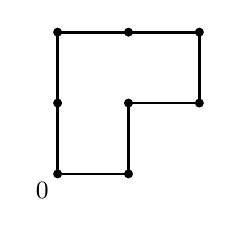
\begin{tikzpicture}[ym/base,x=.90cm,y=.90cm]
  \draw[ym/path] (0,0) -- (1,0) -- (1,1) -- (2,1)
    -- (2,2) -- (0,2) -- cycle;
  \foreach \point in {(0,0),(1,0),(1,1),(2,1),(2,2),(1,2),(0,2),(0,1)}
    \node[ym/dot] at \point {};
  \node[below left,inner sep=3pt] at (0,0) {$0$};
\end{tikzpicture}
\caption{A finite closed path based at the origin.}
\label{fig:wilson-loop}
\end{figure}

\begin{definition}[Correlation functions]
For labels $\nu_1,\ldots,\nu_k$ and sites $x_1,\ldots,x_k$, define
\begin{equation}\label{eq:display-030}
C_{M,\e,\beta}(\nu;x)
 =\int\prod_{j=1}^k\mathcal O_{M,\e}(\nu_j,x_j;U)\,\dd\mu_{\ell,\beta}(U).
\end{equation}
\end{definition}

The first objective is to study $\e\downarrow0$ at fixed $M$.
Set $\ell_{M,\e}=M/\e$ and choose $\beta:=\beta_{M,\e}$ appropriately.

\section{Exact one-step blocking}
With a suitable choice of $\beta_{M,\e}$ and suitable conditions on $\mathcal O_{M,\e}$, the objective is to study
\begin{equation}\label{eq:display-031}
C_{M,\e}(\nu;x):=C_{M,\e,\beta_{M,\e}}(\nu;x)
\end{equation}
as $\e\to0^+$. Locality and continuity alone are not a convergence theorem.

As $\e\to0^+$, the number of integration variables grows. To organize this integral, introduce a coarser configuration.

Write
\begin{equation}\label{eq:display-032}
F(U):=e^{-\beta_{M,\e}W_\ell(U)},
\qquad
O(U)=\prod_{j=1}^k\mathcal O_{M,\e}(\nu_j,x_j;U).
\end{equation}
Then
\begin{equation}\label{eq:display-033}
C_{M,\e}(\nu;x)
 =\frac{\displaystyle\int_{\Uf}O(U)F(U)\,\dd H_{M,\e}(U)}
 {\displaystyle\int_{\Uf}F(U)\,\dd H_{M,\e}(U)}.
\end{equation}
Write $\Uf:=\mathcal U_\ell$ and $\Hf:=H_{M,\e}=H_\ell$; the subscript $\mathrm f$ denotes the fine lattice.

Let $V$ be a coarse configuration with product Haar measure $\dd\Hc(V)$:
\begin{equation}\label{eq:display-034}
V\in\Uc:=G^{E^+_{\ell/L}},\qquad L>1.
\end{equation}
Here $L$ is an integer dividing $\ell$.

Insert the normalization
\begin{equation}\label{eq:blocking-normalization}
1=\int_{\Uc}K(U,V)\,\dd\Hc(V),\qquad\forall U.
\end{equation}
A nonnegative measurable function $K(U,V)$ satisfying~\eqref{eq:blocking-normalization} is called a blocking kernel density.

Thus
\begin{equation}\label{eq:display-036}
\begin{aligned}
\int_{\Uf}O(U)F(U)\,\dd\Hf(U)
&=\int_{\Uf\times\Uc}O(U)F(U)K(U,V)\,\dd\Hc(V)\,\dd\Hf(U)\\
&=\int_{\Uc}\left(\int_{\Uf}O(U)F(U)K(U,V)\,\dd\Hf(U)\right)\dd\Hc(V).
\end{aligned}
\end{equation}
Denote the inner integral by $\Gc(V)$.

Similarly, set
\begin{equation}\label{eq:coarse-density}
\Fc(V):=\int_{\Uf}F(U)K(U,V)\,\dd\Hf(U).
\end{equation}
This gives the \textbf{exact one-step blocking identity}:
\begin{equation}\label{eq:display-038}
C_{M,\e}(\nu;x)
 =\frac{\displaystyle\int_{\Uc}\Gc(V)\,\dd\Hc(V)}
 {\displaystyle\int_{\Uc}\Fc(V)\,\dd\Hc(V)}.
\end{equation}
\begin{equation}\label{eq:display-039}
\text{coarse probability measure:}\qquad
\dd\muc(V)=\frac{\Fc(V)}{Z}\,\dd\Hc(V).
\end{equation}
Here $Z=Z_\ell(\beta_{M,\e})=\int\Fc\,\dd\Hc$, and $\Fc$ is the effective density.

For $\Fc(V)>0$, define
\begin{equation}\label{eq:coarse-observable}
\Oc(V)
:=\frac{\Gc(V)}{\Fc(V)} =\frac{\displaystyle\int_{\Uf}K(U,V)O(U)F(U)\,\dd\Hf(U)}
 {\displaystyle\int_{\Uf}K(U,V)F(U)\,\dd\Hf(U)}.
\end{equation}
Therefore
\begin{equation}\label{eq:display-041}
C_{M,\e}(\nu;x)=\int_{\Uc}\Oc(V)\,\dd\muc(V).
\end{equation}

\section{A two-dimensional example}

For this example, consider a single square coarse plaquette $P$ of mesh $\e$ in two dimensions.
Subdivide $P$ into $L^2$ fine plaquettes, as illustrated schematically in Figure~\ref{fig:fine-coarse}. The fine mesh is
\begin{equation}\label{eq:display-042}
\delta=\e/L.
\end{equation}

\begin{figure}[htbp]
\centering
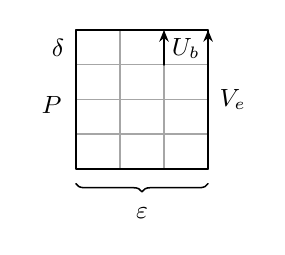
\begin{tikzpicture}[ym/base,x=.56cm,y=.44cm]
  \foreach \x in {0,1,2,3}
    \draw[ym/grid] (\x,0) -- (\x,4);
  \foreach \y in {0,1,2,3,4}
    \draw[ym/grid] (0,\y) -- (3,\y);
  \draw[ym/edge] (0,0) rectangle (3,4);
  \draw[ym/arrow] (2,3) -- (2,4);
  \node[anchor=west,inner sep=2pt] at (2.04,3.48) {$U_b$};
  \draw[ym/arrow] (3,0) -- (3,4);
  \node[anchor=west,inner sep=4pt] at (3,2) {$V_e$};
  \node[anchor=east,inner sep=4pt] at (0,3.50) {$\delta$};
  \node[anchor=east,inner sep=5pt] at (0,1.85) {$P$};
  \draw[ym/brace] (0,-.43) -- (3,-.43)
    node[midway,below=5pt] {$\varepsilon$};
\end{tikzpicture}
\caption{Fine links and a coarse boundary link of a plaquette $P$ (schematic).}
\label{fig:fine-coarse}
\end{figure}

On the fine edges in $P$, put the Wilson measure
\begin{equation}\label{eq:display-043}
\mu_\delta(\dd U)=\frac1{Z_\delta}\prod_{q\in\mathcal P}Q_\delta(U_q)
\prod_{b\in E_\delta^+}\dd U_b,
\qquad
Q_\delta(U)\propto\exp\left(-\beta\left(1-\frac1N\operatorname{Re}\tr U\right)\right).
\end{equation}
Define
\begin{equation}\label{eq:display-044}
V_e=U_{b_1}\cdots U_{b_L},
\qquad\Pi_L:U\longmapsto V.
\end{equation}
We compute the pushforward $(\Pi_L)_*\mu_\delta$. In this example $\Gc$ is a bounded test function, $\mathcal P$ is the set of fine plaquettes in $P$, and $\partial E_\delta^+$ consists of the fine boundary edges.
\begin{equation}\label{eq:display-045}
\begin{aligned}
\int\Gc(V)\,(\Pi_L)_*\mu_\delta(\dd V)
&=\int\Gc(\Pi_LU)\,\mu_\delta(\dd U)\\
&\propto\int\Gc(\Pi_LU)\prod_{q\in\mathcal P}Q_\delta(U_q)
 \prod_{b\in E_\delta^+}\dd U_b\\
&\propto\int\Gc(\Pi_LU)
 \left(\int_{G^{E_\delta^+\setminus\partial E_\delta^+}}
 \prod_{q\in\mathcal P}Q_\delta(U_q)
 \prod_{b\in E_\delta^+\setminus\partial E_\delta^+}\dd U_b\right)
 \prod_{b\in\partial E_\delta^+}\dd U_b.
\end{aligned}
\end{equation}

The elementary merging identity is illustrated in Figure~\ref{fig:merging}.
\begin{figure}[htbp]
\centering
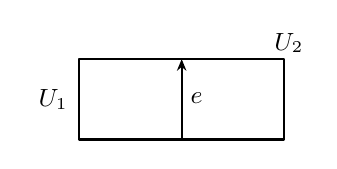
\begin{tikzpicture}[ym/base]
  \draw[ym/edge] (0,0) rectangle (2.60,1.02);
  \draw[ym/arrow] (1.30,0) -- (1.30,1.02);
  \node[anchor=west,inner sep=3pt] at (1.30,.53) {$e$};
  \node[anchor=east,inner sep=4pt] at (0,.51) {$U_1$};
  \node[anchor=south west,inner sep=2pt] at (2.40,1.02) {$U_2$};
\end{tikzpicture}
\caption{Two adjacent plaquettes sharing the link $e$.}
\label{fig:merging}
\end{figure}

\begin{equation}\label{eq:display-046}
\int_GQ_\delta(U_1U_e^{-1})Q_\delta(U_eU_2)\,\dd U_e =(Q_\delta*Q_\delta)(U_1U_2).
\end{equation}
Only the outer boundary holonomy remains. Here $(f*g)(W):=\int_G f(WV^{-1})g(V)\,\dd h_G(V)$ denotes convolution.

Consequently,
\begin{equation}\label{eq:display-047}
\int_{G^{E_\delta^+\setminus\partial E_\delta^+}}
\prod_{q\in\mathcal P}Q_\delta(U_q)
\prod_{b\in E_\delta^+\setminus\partial E_\delta^+}\dd U_b
=K_{\delta,P}\bigl(U(\partial P)\bigr).
\end{equation}
The function $K_{\delta,P}$ depends only on the boundary holonomy of $P$.

Therefore
\begin{equation}\label{eq:display-048}
\begin{aligned}
\int\Gc(V)\,(\Pi_L)_*\mu_\delta(\dd V)
&\propto\int\Gc(\Pi_LU)K_{\delta,P}\bigl(U(\partial P)\bigr)
\prod_{b\in\partial E_\delta^+}\dd U_b\\
&=\int\Gc(V)K_{\delta,P}\bigl(V(\partial P)\bigr)
(\Pi_L)_*\left(\prod_{b\in\partial E_\delta^+}\dd U_b\right)(\dd V).
\end{aligned}
\end{equation}
Here
\begin{equation}\label{eq:display-049}
(\Pi_L)_*\left(\prod_{b\in\partial E_\delta^+}\dd U_b\right)(\dd V)
=\prod_{e\in E_\e^+}\dd V_e.
\end{equation}
This is deterministic blocking, described by the probability kernel
\begin{equation}\label{eq:display-050}
K(U,\dd V)=\delta_{\Pi_L(U)}(\dd V).
\end{equation}

\section{A smooth blocking kernel}
Return to four dimensions. We now choose a blocking density so that $V$ records local information about $U$.

Compare the noise normalization and kernel in
\cite[Section~11, (11.1)--(11.2), p.~36]{Exposition}.
Here we use a single straight-path predictor.\par\smallskip

\subsection{Coarse-link holonomy}

The coarse link from $x$ to $x+e_i$ corresponds to a fine path from $Lx$ to $Lx+Le_i$; see Figure~\ref{fig:coarse-link}.

\begin{figure}[htbp]
\centering
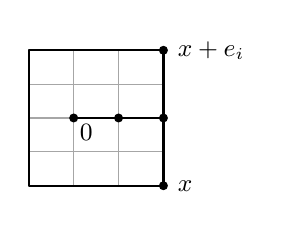
\begin{tikzpicture}[ym/base,x=.57cm,y=.43cm]
  \foreach \x in {0,1,2,3}
    \draw[ym/grid] (\x,0) -- (\x,4);
  \foreach \y in {0,1,2,3,4}
    \draw[ym/grid] (0,\y) -- (3,\y);
  \draw[ym/edge] (0,0) rectangle (3,4);
  \draw[ym/path] (1,2) -- (3,2);
  \draw[ym/path] (3,0) -- (3,4);
  \foreach \point in {(1,2),(2,2),(3,2),(3,0),(3,4)}
    \node[ym/dot] at \point {};
  \node[below right,inner sep=2pt] at (1,2) {$0$};
  \node[anchor=west,inner sep=5pt] at (3,0) {$x$};
  \node[anchor=west,inner sep=5pt] at (3,4) {$x+e_i$};
\end{tikzpicture}
\caption{A coarse link and its fine-lattice realization (schematic).}
\label{fig:coarse-link}
\end{figure}

\begin{equation}\label{eq:display-051}
Q(U)_i(x):=U_i(Lx)U_i(Lx+e_i)\cdots U_i\bigl(Lx+(L-1)e_i\bigr).
\end{equation}
Allow $V$ to fluctuate around $Q(U)$.

The mismatch is
\begin{equation}\label{eq:display-052}
V_eQ(U)_e^{-1}\qquad\text{(mismatch)}.
\end{equation}
For $W\in G$, set
\begin{equation}\label{eq:display-053}
q_G(W):=1-\frac1N\operatorname{Re}\tr W =\frac1{2N}\|W-I\|_{\mathrm{HS}}^2\ge0.
\end{equation}
Assign to this mismatch the weight
\begin{equation}\label{eq:display-054}
\exp\left(-a\beta\,q_G\bigl(V_eQ(U)_e^{-1}\bigr)\right).
\end{equation}
Here $a>0$ is fixed and $\beta:=\beta_{M,\e}>0$.
The weight is maximal when $V_e=Q(U)_e$. The Hilbert--Schmidt norm is $\|B\|_{\mathrm{HS}}^2=\tr(BB^*)$.

Define
\begin{equation}\label{eq:display-055}
z_n(\beta):=\int_Ge^{-a\beta q_G(W)}\,\dd h_G(W)\in[e^{-a\beta},1].
\end{equation}

\begin{equation}\label{eq:smooth-kernel}
K_\beta(U,V):=\prod_{e\in E_{\ell/L}^+}
\frac{e^{-a\beta q_G(V_eQ(U)_e^{-1})}}{z_n(\beta)}.
\end{equation}
Right invariance of Haar measure gives
\begin{equation}\label{eq:display-057}
\int_Ge^{-a\beta q_G(V_eQ(U)_e^{-1})}\,\dd V_e
=\int_Ge^{-a\beta q_G(W)}\,\dd W =z_n(\beta).
\end{equation}
Thus
\begin{equation}\label{eq:display-058}
\int_{\Uc}K_\beta(U,V)\,\dd\Hc(V)=1.
\end{equation}
\begin{remark} At fixed $\beta>0$, as $a\to\infty$,
\begin{equation}\label{eq:display-059}
K_{\beta,a}(U,V)\,\dd\Hc(V)\Longrightarrow\delta_{Q(U)}(\dd V).
\end{equation}
\end{remark}

The coarse density is therefore
\begin{equation}\label{eq:display-060}
\begin{aligned}
\Fc(V)
&=\int_{\mathcal U_\ell}K_\beta(U,V)e^{-\beta W_\ell(U)}\,\dd\Hf(U)\\
&=z_n(\beta)^{-\#E_{\ell/L}^+}\int_{\Uf}
\exp\left\{-\beta\left[W_\ell(U)
+a\sum_{e\in E_{\ell/L}^+}q_G\bigl(V_eQ(U)_e^{-1}\bigr)\right]\right\}
\dd\Hf(U).
\end{aligned}
\end{equation}
\section{Tree gauge}
We follow \cite[Section~11, Lemma~11.2, p.~37]{Exposition}.

Set
\begin{equation}\label{eq:blocking-action}
A(V,U):=W_\ell(U)+a\sum_{e\in E_{\ell/L}^+}q_G\bigl(V_eQ(U)_e^{-1}\bigr).
\end{equation}
The path products transform according to
\begin{equation}\label{eq:display-062}
Q(U^g)_i(x)=g(Lx)Q(U)_i(x)g(Lx+Le_i)^{-1}.
\end{equation}

If $g(Lx)=1$ at every embedded coarse site, then
\begin{equation}\label{eq:display-063}
Q(U^g)=Q(U)
\quad\Longrightarrow\quad
A(V,U^g)=A(V,U).
\end{equation}
We now integrate out the gauge freedom in
\begin{equation}\label{eq:display-064}
\int_{\Uf}\exp\bigl(-A(V,U)\bigr)\,\dd\Hf(U)
\end{equation}
by fixing the links of a rooted tree in each block.

\begin{figure}[htbp]
\centering
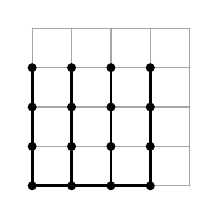
\begin{tikzpicture}[ym/base,x=.50cm,y=.50cm]
  \foreach \x in {0,1,2,3,4}
    \draw[ym/grid] (\x,0) -- (\x,4);
  \foreach \y in {0,1,2,3,4}
    \draw[ym/grid] (0,\y) -- (4,\y);
  \draw[ym/path] (0,0) -- (3,0);
  \foreach \x in {0,1,2,3}
    \draw[ym/path] (\x,0) -- (\x,3);
  \foreach \x in {0,1,2,3}
    \foreach \y in {0,1,2,3}
      \node[ym/dot] at (\x,\y) {};
\end{tikzpicture}
\caption{A rooted block tree, shown in two dimensions; dark edges form the tree.}
\label{fig:block-tree}
\end{figure}

In each coarse block $Lx+\{0,\ldots,L-1\}^4$, choose a tree such that
\begin{enumerate}[label=(\roman*)]
\item its vertices are exactly $Lx+\{0,\ldots,L-1\}^4$;
\item its root is $Lx$.
\end{enumerate}
Any such tree suffices for this identity; Figure~\ref{fig:block-tree} shows a two-dimensional example.
Let $T$ denote the union of their edges, represented with the positive lattice orientation.

\begin{definition}[Tree gauge] $U$ is in tree gauge if $U|_T=\id$.

\end{definition}

\begin{lemma}\label{lem:tree-gauge} Every configuration can be transformed into tree gauge by a gauge transformation.\end{lemma}

\begin{proof} Consider $U\in\Uf$. Set $g=\id$ at each root.
Suppose $g(x)$ has been determined at a parent $x$. Write $U_{xy}$ for the link from $x$ to its child $y$, using the inverse if this reverses the positive lattice orientation. Define
\begin{equation}\label{eq:display-065}
g(y):=g(x)U_{xy},\qquad\forall y\text{ such that }y\text{ has parent }x.
\end{equation}
Then
\begin{equation}\label{eq:display-066}
U_{xy}^g
=g(x)U_{xy}g(y)^{-1} =g(x)U_{xy}\bigl(g(x)U_{xy}\bigr)^{-1} =\id.
\end{equation}
\end{proof}

Write
\begin{equation}\label{eq:remaining-links}
I:=E_\ell^+\setminus T.
\end{equation}
Writing $e_-,e_+$ for the initial and terminal vertices of $e$, the remaining configuration is determined by
\begin{equation}\label{eq:display-068}
u_e:=g(e_-)U_eg(e_+)^{-1},\qquad e\in I
\end{equation}

For $u\in G^I$, define
\begin{equation}\label{eq:display-069}
U_T(u)_e=
\begin{cases}
1,&e\in T,\\
u_e,&e\in I.
\end{cases}
\end{equation}
To integrate out the links in $T$, write
\begin{equation}\label{eq:display-070}
J(U):=\exp\bigl(-A(V,U)\bigr).
\end{equation}
Then
\begin{equation}\label{eq:display-071}
\begin{aligned}
\int_{\Uf}J(U)\,\dd\Hf(U)
&=\int_{\Uf}J\bigl(U_T(u)\bigr)\,\dd\Hf(U)
\qquad\text{by gauge invariance}\\
&=\int_{G^T}\left(\int_{G^I}J\bigl(U_T(u)\bigr)
\prod_{e\in I}\dd U_e\right)\prod_{e\in T}\dd U_e.
\end{aligned}
\end{equation}
For each fixed collection of tree links, $g$ depends only on those links. Under the change of variables
\begin{equation}\label{eq:display-072}
U_e\longmapsto u_e=g(e_-)U_eg(e_+)^{-1}
\end{equation}
left and right Haar invariance give $\dd U_e=\dd u_e$ for $e\in I$. The normalized integral over $G^T$ is one, so the expression equals
\begin{equation}\label{eq:display-073}
\int_{G^I}J\bigl(U_T(u)\bigr)\prod_{e\in I}\dd u_e.
\end{equation}
Write $\dd h_G^I(u)=\prod_{e\in I}\dd u_e$.

Consequently,
\begin{equation}\label{eq:display-074}
\int_{\Uf}J(U)\,\dd\Hf(U)
=\int_{G^I}J\bigl(U_T(u)\bigr)\prod_{e\in I}\dd u_e.
\end{equation}

It follows that
\begin{equation}\label{eq:display-075}
\boxed{
\Fc(V)=z_n(\beta)^{-\#E_{\ell/L}^+}
\int_{G^I}e^{-\beta A(V,U_T(u))}\,\dd h_G^I(u).
}
\end{equation}
\section{Exponential coordinates and sectors}
We express the remaining group-valued links in local exponential coordinates.

Near the identity, write $U=e^X$. Equip $\g$ with the inner product $\langle X,Y\rangle_\g=\operatorname{Re}\tr(X^*Y)$ and $G$ with the induced left-invariant Riemannian metric. Then
\begin{equation}\label{eq:display-076}
\boxed{
\dd h_G(e^X)=\zeta_Gj_G(X)\,\dd X,\qquad |X|_{\g}<r_G.
}
\end{equation}
Here
\begin{equation}\label{eq:display-077}
\zeta_G=\frac1{\Vol(G)},
\end{equation}
$r_G>0$ is such that $X\mapsto e^X$ is a diffeomorphism onto its image for $|X|_\g<r_G$,
\begin{equation}\label{eq:display-078}
j_G(X)=\left|\det_{\g}\left(\int_0^1e^{-t\ad X}\,\dd t\right)\right|,
\qquad(\ad X)Y:=[X,Y].
\end{equation}
\begin{remark} $j_G>0$ and is smooth on $|X|_\g<r_G$.
\begin{equation}\label{eq:display-079}
j_G(0)=1.
\end{equation}
\end{remark}

\begin{remark} For $G=U(1)$, $j_G(X)\equiv1$.\end{remark}

The volume formula is derived in Appendix~\ref{sec:haar-appendix}.

Choose a smooth $\chi:G\to[0,1]$ supported inside the image of $\{X:|X|_\g<r_G\}$. Then
\begin{equation}\label{eq:display-080}
\int_G\chi(U)f(U)\,\dd h_G(U)
=\zeta_G\int_{|X|_\g<r_G}\chi(e^X)f(e^X)j_G(X)\,\dd X.
\end{equation}
The full integral splits exactly as
\begin{equation}\label{eq:display-081}
\int_Gf\,\dd h_G
=\int_G\chi f\,\dd h_G+\int_G(1-\chi)f\,\dd h_G.
\end{equation}

\begin{remark} To describe fluctuations around a fixed reference link $R\in G$, write
\begin{equation}\label{eq:display-082}
U=e^XR.
\end{equation}
Right invariance gives
\begin{equation}\label{eq:display-083}
\dd h_G(e^XR)=\zeta_Gj_G(X)\,\dd X.
\end{equation}
\end{remark}

For the fluctuation-integral organization, compare \cite[Section~2, pp.~265--268]{Bal87}.

Apply this to the integral
\begin{equation}\label{eq:display-084}
\int_{G^I}e^{-\beta A(V,U_T(u))}\,\dd h_G^I(u).
\end{equation}
The cutoff decomposition is an exact identity.

Fix $V$ and choose a reference link for each $e\in I$:
\begin{equation}\label{eq:display-085}
R_e(V)\in G.
\end{equation}
Split each link factor as
\begin{equation}\label{eq:display-086}
1=\chi\bigl(U_eR_e(V)^{-1}\bigr)
+\left[1-\chi\bigl(U_eR_e(V)^{-1}\bigr)\right].
\end{equation}
On the support of the first term, $U_e$ has the unique representation
\begin{equation}\label{eq:display-087}
\exists y_e\in\{X\in\g:|X|_\g<r_G\}\quad\text{s.t.}\quad U_e=e^{y_e}R_e(V).
\end{equation}
Multiplying over $e\in I$ gives
\begin{equation}\label{eq:display-088}
\begin{aligned}
1&=\prod_{e\in I}\left(\chi\bigl(U_eR_e(V)^{-1}\bigr)
+\left[1-\chi\bigl(U_eR_e(V)^{-1}\bigr)\right]\right)\\
&=\sum_{\Ia\subset I}
\prod_{e\in\Ia}\chi\bigl(U_eR_e(V)^{-1}\bigr)
\prod_{e\in\If=I\setminus\Ia}\left[1-\chi\bigl(U_eR_e(V)^{-1}\bigr)\right].
\end{aligned}
\end{equation}
The links in $\Ia$ are called active, and those in $\If=I\setminus\Ia$ are called frozen.

Each term is called a sector. Fix $\Ia,\If$ and write
\begin{equation}\label{eq:display-089}
U_e=
\begin{cases}
e^{y_e}R_e(V),&\text{for some }y_e\in\{X\in\g:|X|_\g<r_G\},\quad e\in\Ia,\\
Y_e,&e\in\If.
\end{cases}
\end{equation}
The full configuration is
\begin{equation}\label{eq:display-090}
U(V,Y,y)_e=
\begin{cases}
1,&e\in T,\\
e^{y_e}R_e(V),&e\in\Ia,\\
Y_e,&e\in\If.
\end{cases}
\end{equation}
For the active links, the change of variables gives
\begin{equation}\label{eq:display-091}
\dd h_G(U_e)=\zeta_Gj_G(y_e)\,\dd y_e,\qquad e\in\Ia.
\end{equation}
Therefore
\begin{equation}\label{eq:display-092}
\dd h_G(u)=\zeta_G^{|\Ia|}
\left(\prod_{e\in\Ia}j_G(y_e)\right)\dd y\,\dd h_G^{\If}(Y),
\qquad\dd y=\prod_{e\in\Ia}\dd y_e.
\end{equation}
Substituting $U(V,Y,y)$ into the action, set
\begin{equation}\label{eq:sector-action}
\varphi(V,Y,y):=A\bigl(V,U(V,Y,y)\bigr),
\end{equation}
\begin{equation}\label{eq:sector-cutoff}
\Theta(V,Y,y):=
\prod_{e\in\Ia}\chi(e^{y_e})
\prod_{e\in\If}\left[1-\chi\bigl(Y_eR_e(V)^{-1}\bigr)\right].
\end{equation}
Write
\begin{equation}\label{eq:display-095}
\prod_{e\in\Ia}j_G(y_e)
=\exp\left(\sum_{e\in\Ia}\log j_G(y_e)\right).
\end{equation}

Write
\begin{equation}\label{eq:haar-correction}
\psi(V,Y,y):=-\sum_{e\in\Ia}\log j_G(y_e)
\qquad\text{(Haar correction)}.
\end{equation}
% User-approved local amendment: make the chart domain explicit.
Choose an orthonormal basis of $\g$ and identify the active coordinates with $\R^d$, where $d:=|\Ia|\dim_{\R}\g$. The chart domain is
\begin{equation}\label{eq:chart-domain}
\boxed{
\Omega:=\left\{y\in\g^{\Ia}:|y_e|_{\g}<r_G
\text{ for every }e\in\Ia\right\}\subset\R^d.
}
\end{equation}
The contribution of this sector to the tree-gauge integral is
\begin{equation}\label{eq:display-098}
\zeta_G^{|\Ia|}\int_{G^{\If}}\dd h_G^{\If}(Y)
\int_{\Omega}\Theta(V,Y,y)e^{-(\beta\varphi+\psi)(V,Y,y)}\,\dd y.
\end{equation}
\section{Rewriting the integral as a Gaussian expectation}
Fix the coarse configuration $V$ and the frozen variables $Y$, and suppress them in the notation.

The active-coordinate integral is
\begin{equation}\label{eq:display-099}
\int_{\Omega}\Theta(y)e^{-(\beta\varphi+\psi)(y)}\,\dd y.
\end{equation}
To extract a Gaussian part, use the following identity.

\begin{lemma}[Gaussian change of variables]\label{lem:gaussian-change}
Let $B\in L^1(\R^d)$, $g>0$, $m\in\R^d$, and let $C$ be a symmetric positive-definite matrix. Then
\begin{equation}\label{eq:gaussian-identity}
\int_{\R^d}B(y)\,\dd y
=(2\pi g^2)^{d/2}(\det C)^{1/2} \times\int_{\R^d}
 e^{\frac12z^{\mathsf T}C^{-1}z}B(m+gz)\,\dd\mu_C(z),
\end{equation}

Here $\mu_C=\mathcal N(0,C)$.

\end{lemma}

Taking $g:=\beta^{-1/2}$ gives
\begin{equation}\label{eq:display-101}
\begin{aligned}
&\int_{\Omega}\Theta(y)e^{-(\beta\varphi+\psi)(y)}\,\dd y\\
&=\int_{\{z\in\R^d:\,m+gz\in\Omega\}}\Theta(m+gz)\\
&\qquad\times\exp\left\{-g^{-2}\varphi(m+gz)-\psi(m+gz)
+\frac12z^{\mathsf T}C^{-1}z\right\}\,\dd\mu_C(z)
\times(2\pi g^2)^{d/2}(\det C)^{1/2}.
\end{aligned}
\end{equation}
The intended choice of $m$ removes the linear term, while $C$ matches the quadratic term.

We keep $V,Y$ fixed throughout the following calculation.
Write $\mathcal P_\ell^+$ for the positively oriented plaquettes, indexed by
$x\in\Lambda_\ell$ and $1\le i<j\le4$. Recall that
\begin{equation}\label{eq:expanded-sector-action}
\begin{aligned}
\varphi(y)
&=W_\ell\bigl(U(V,Y,y)\bigr)
+a\sum_{e\in E_{\ell/L}^+}q_G\bigl(V_eQ(U)_e^{-1}\bigr)\\
&=\sum_{p\in\mathcal P_\ell^+}
\left(1-\frac1N\operatorname{Re}\tr P_p(U)\right)
+a\sum_{e\in E_{\ell/L}^+}q_G\bigl(V_eQ(U)_e^{-1}\bigr),
\end{aligned}
\end{equation}
where $U=U(V,Y,y)$, while
\begin{equation}\label{eq:recalled-haar-correction}
\psi(y)=-\sum_{e\in\Ia}\log j_G(y_e).
\end{equation}
The existence of a stationary centre and the required Hessian bounds are
model-dependent inputs. For now, assume that $m\in\Omega$ satisfies
\begin{equation}\label{eq:stationary-centre-input}
D_y\varphi(m)=0,\qquad
H:=D_y^2\varphi(m)>0,\qquad C=H^{-1}.
\end{equation}
These assumptions will be retained explicitly in the estimates below.

\subsection{Matching the linear and quadratic terms}
For $m+gz\in\Omega$, set $f(t):=\varphi(m+tgz)$. Then
\begin{equation}\label{eq:line-derivatives}
f'(t)=gD_y\varphi(m+tgz)[z],\qquad
f''(t)=g^2D_y^2\varphi(m+tgz)[z,z].
\end{equation}
Taylor's formula gives
\begin{equation}\label{eq:line-taylor-formula}
\begin{aligned}
\varphi(m+gz)-\varphi(m)
&=gD_y\varphi(m)[z]\\
&\quad+g^2\int_0^1(1-t)D_y^2\varphi(m+tgz)[z,z]\,\dd t.
\end{aligned}
\end{equation}
The first term vanishes by \eqref{eq:stationary-centre-input}. Define
\begin{equation}\label{eq:taylor-quadratic-integral}
V_g(z):=\int_0^1(1-t)D_y^2\varphi(m+tgz)[z,z]\,\dd t,
\qquad V_0(z)=\frac12z^{\mathsf T}Hz.
\end{equation}
Since $C^{-1}=H$, the exponent in the Gaussian change of variables becomes
\begin{equation}\label{eq:matched-exponent}
\begin{aligned}
&-g^{-2}\varphi(m+gz)-\psi(m+gz)
+\frac12z^{\mathsf T}C^{-1}z\\
&=-g^{-2}\bigl(\varphi(m)+g^2V_g(z)\bigr)-\psi(m+gz)+V_0(z)\\
&=-g^{-2}\varphi(m)-\psi(m)
+V_0(z)-V_g(z)+\psi(m)-\psi(m+gz).
\end{aligned}
\end{equation}
Thus the remaining correction is
\begin{equation}\label{eq:remaining-exponent}
V_0(z)-V_g(z)+\psi(m)-\psi(m+gz).
\end{equation}
Only $\varphi$ carries the factor $g^{-2}$. Matching its quadratic term
therefore removes an order-one fluctuation term; the smooth Haar correction
can remain in the residual exponent.

Substitution into \eqref{eq:display-101} yields
\begin{equation}\label{eq:full-gaussian-representation}
\begin{aligned}
&\int_\Omega\Theta(y)e^{-g^{-2}\varphi(y)-\psi(y)}\,\dd y\\
&=(2\pi g^2)^{d/2}(\det H)^{-1/2}
e^{-g^{-2}\varphi(m)-\psi(m)}\\
&\quad\times\int_{\{z:\,m+gz\in\Omega\}}
\Theta(m+gz)
e^{V_0(z)-V_g(z)+\psi(m)-\psi(m+gz)}\,\dd\mu_C(z).
\end{aligned}
\end{equation}
Write the last integral as
\begin{equation}\label{eq:full-Z}
Z(g):=\int_{\{z:\,m+gz\in\Omega\}}
\Theta(m+gz)
e^{V_0(z)-V_g(z)+\psi(m)-\psi(m+gz)}\,\dd\mu_C(z).
\end{equation}
\begin{remark}
The Hessian varies with $V,Y$, so its determinant must be retained.
The reference Gaussian is a measure on $\R^d$, but the transformed chart
domain and the actual cutoff remain in \eqref{eq:full-Z}.
\end{remark}

\section{The central Gaussian integral}\label{sec:central-estimates}
We first estimate an auxiliary integral on a symmetric ball, before restoring
the sector cutoff. Choose a fluctuation radius $D>0$. For $g>0$,
\begin{equation}\label{eq:central-ball-coordinates}
|z|\le D\quad\Longleftrightarrow\quad |y-m|\le gD.
\end{equation}
Whenever the entire trajectory $m+tgz$, $0\le t\le1$, stays in the smooth
chart, define
\begin{equation}\label{eq:central-Z-definition}
Z_D(g):=\int_{|z|\le D}
e^{V_0(z)-V_g(z)+\psi(m)-\psi(m+gz)}\,\dd\mu_C(z).
\end{equation}
We also use this formula for negative $g$ near zero. The target is
\begin{equation}\label{eq:central-target}
\log Z_D(g)-\log Z_D(0)=O(g^2).
\end{equation}
For the corresponding calculation with coarse derivatives and a moving
determinant, compare \cite[Section~12, Theorem~12.5, pp.~42--43]{Exposition}.
Here $V,Y,m,C,\varphi,\psi$ are held fixed when differentiating in $g$.

\subsection{Cancellation of the first derivative}
Under the smoothness assumptions stated below, at $g=0$,
\begin{equation}\label{eq:central-zero-mass}
Z_D(0)=\int_{|z|\le D}1\,\dd\mu_C(z).
\end{equation}
Differentiating the Taylor integral gives
\begin{equation}\label{eq:first-taylor-g-derivative}
\begin{aligned}
\partial_gV_g(z)
&=\partial_g\int_0^1(1-t)D_y^2\varphi(m+tgz)[z,z]\,\dd t\\
&=\int_0^1t(1-t)D_y^3\varphi(m+tgz)[z,z,z]\,\dd t.
\end{aligned}
\end{equation}
In particular,
\begin{equation}\label{eq:first-taylor-at-zero}
\left.\partial_gV_g(z)\right|_{g=0}
=\frac16D_y^3\varphi(m)[z,z,z].
\end{equation}
Consequently,
\begin{equation}\label{eq:central-first-derivative}
Z_D'(0)=\int_{|z|\le D}
\left(-\frac16D_y^3\varphi(m)[z,z,z]-D_y\psi(m)[z]\right)\,\dd\mu_C(z)=0.
\end{equation}
The integrand is odd in $z$, whereas both the ball and the centred Gaussian
measure are invariant under $z\mapsto-z$.

\subsection{A bound on the second derivative}
Assume there is a common $g_*>0$ such that, for all parameters under
consideration,
\begin{equation}\label{eq:common-central-neighbourhood}
m+tgz\in\Omega,
\qquad |z|\le D,\quad 0\le t\le1,\quad |g|\le g_*.
\end{equation}
For the active chart factors, also suppose that
$e^{(m+tgz)_e}\in\operatorname{supp}\chi$ on these trajectories.
Suppose $\varphi$ is $C^4$ and $\psi$ is $C^2$ in a common neighbourhood
of these points, and that, for a common $K_*\ge1$,
\begin{equation}\label{eq:central-derivative-inputs}
\|D_y^3\varphi\|_{\mathrm{op}},\quad
\|D_y^4\varphi\|_{\mathrm{op}},\quad
\|D_y\psi\|_{\mathrm{op}},\quad
\|D_y^2\psi\|_{\mathrm{op}}\le K_*.
\end{equation}
The operator norms here are those of multilinear forms on the active
Euclidean coordinate space. Their validity for the chosen reference links,
stationary centre and Hessian remains a model-dependent task.

\begin{lemma}[Second derivative of the central logarithm]\label{lem:central-log-second}
Under \eqref{eq:common-central-neighbourhood}--\eqref{eq:central-derivative-inputs},
there is $B=B(K_*,D)$ such that
\begin{equation}\label{eq:central-log-second}
\sup_{V,Y}\sup_{|g|\le g_*}
\left|\partial_g^2\log Z_D(g;V,Y)\right|\le2B.
\end{equation}
\end{lemma}
\begin{proof}
Set
\begin{equation}\label{eq:central-P-definition}
P_g(z):=V_0(z)-V_g(z)+\psi(m)-\psi(m+gz).
\end{equation}
Then
\begin{equation}\label{eq:central-P-zero}
Z_D(g)=\int_{|z|\le D}e^{P_g(z)}\,\dd\mu_C(z),\qquad P_0(z)=0.
\end{equation}
A second differentiation gives
\begin{equation}\label{eq:second-taylor-g-derivative}
\partial_g^2V_g(z)
=\int_0^1t^2(1-t)D_y^4\varphi(m+tgz)[z,z,z,z]\,\dd t.
\end{equation}
Hence
\begin{equation}\label{eq:taylor-g-derivative-bounds}
|\partial_gV_g(z)|\le\frac16K_*|z|^3,\qquad
|\partial_g^2V_g(z)|\le\frac1{12}K_*|z|^4.
\end{equation}
Similarly,
\begin{equation}\label{eq:haar-g-derivative-bounds}
|\partial_g\psi(m+gz)|\le K_*|z|,\qquad
|\partial_g^2\psi(m+gz)|\le K_*|z|^2.
\end{equation}
On $|z|\le D$ this implies
\begin{equation}\label{eq:central-P-derivative-bounds}
\begin{aligned}
|\partial_gP_g(z)|&\le K_*\left(\frac{D^3}{6}+D\right),\\
|\partial_g^2P_g(z)|&\le K_*\left(\frac{D^4}{12}+D^2\right).
\end{aligned}
\end{equation}
Since $P_0=0$,
\begin{equation}\label{eq:central-P-value-bound}
|P_g(z)|\le g_*K_*\left(\frac{D^3}{6}+D\right).
\end{equation}
These common bounds justify differentiation under the integral and give
\begin{equation}\label{eq:central-Z-derivative-bounds}
\begin{aligned}
|Z_D'(g)|&\le K_*\left(\frac{D^3}{6}+D\right)Z_D(g),\\
|Z_D''(g)|&\le
\left[K_*\left(\frac{D^4}{12}+D^2\right)
+K_*^2\left(\frac{D^3}{6}+D\right)^2\right]Z_D(g).
\end{aligned}
\end{equation}
The integral is strictly positive, and its ratio to $Z_D(0)$ is bounded
above and below by the exponentials of the right side of
\eqref{eq:central-P-value-bound}. Using
\begin{equation}\label{eq:log-second-identity}
\partial_g^2\log Z_D(g)
=\frac{Z_D''(g)}{Z_D(g)}
-\left(\frac{Z_D'(g)}{Z_D(g)}\right)^2,
\end{equation}
we obtain \eqref{eq:central-log-second}, for example with
\begin{equation}\label{eq:central-B-choice}
2B=K_*\left(\frac{D^4}{12}+D^2\right)
+2K_*^2\left(\frac{D^3}{6}+D\right)^2.
\end{equation}
\end{proof}
Combining this bound with $Z_D'(0)=0$ proves
\begin{equation}\label{eq:central-log-quadratic}
|\log Z_D(g)-\log Z_D(0)|\le B(K_*,D)g^2.
\end{equation}

\subsection{The Gaussian mass at zero coupling}
We now estimate $\log Z_D(0)$. Assume a common spectral lower bound
\begin{equation}\label{eq:uniform-spectral-input}
H(V,Y)\ge\eta\,\mathrm{Id},\qquad\eta>0.
\end{equation}
Since $C=H^{-1}$, we have $C\le\eta^{-1}\mathrm{Id}$ and
$C_{ii}\le\eta^{-1}$ for every coordinate.

\begin{lemma}[Gaussian ball tail]\label{lem:gaussian-ball-tail}
Let $d\ge1$, $C=H^{-1}$ and $H\ge\eta\,\mathrm{Id}$. Then
\begin{equation}\label{eq:zero-coupling-tail}
1-Z_D(0)\le2d\exp\left(-\frac{\eta D^2}{2d}\right).
\end{equation}
If the right side is at most $1/2$, then
\begin{equation}\label{eq:zero-coupling-log-bound}
|\log Z_D(0)|\le4d\exp\left(-\frac{\eta D^2}{2d}\right).
\end{equation}
\end{lemma}
\begin{proof}
For $Z\sim\mathcal N(0,C)$, the one-dimensional Gaussian tail bound gives
\begin{equation}\label{eq:coordinate-gaussian-tail}
\mathbb P\left(|Z_i|>\frac D{\sqrt d}\right)
\le2\exp\left(-\frac{\eta D^2}{2d}\right).
\end{equation}
If $|Z|>D$, at least one coordinate satisfies $|Z_i|>D/\sqrt d$.
The union bound therefore gives
\begin{equation}\label{eq:gaussian-tail-union}
\begin{aligned}
1-Z_D(0)&=\mathbb P(|Z|>D)\\
&\le\sum_{i=1}^d\mathbb P\left(|Z_i|>\frac D{\sqrt d}\right)\\
&\le2d\exp\left(-\frac{\eta D^2}{2d}\right).
\end{aligned}
\end{equation}
If this bound is at most $1/2$, then $Z_D(0)\ge1/2$, and
\begin{equation}\label{eq:gaussian-mass-log-calculation}
\begin{aligned}
|\log Z_D(0)|&=-\log Z_D(0)
=\int_{Z_D(0)}^1\frac{\dd t}{t}\\
&\le2(1-Z_D(0))
\le4d\exp\left(-\frac{\eta D^2}{2d}\right).
\end{aligned}
\end{equation}
\end{proof}

\subsection{The combined conditional estimate}
The inputs can now be collected as follows.
\begin{enumerate}[label=(\roman*)]
\item For every $V,Y$ under consideration, there is a stationary centre
$m(V,Y)$ satisfying
\begin{equation}\label{eq:combined-stationary-input}
D_y\varphi(V,Y,m)=0,\qquad
H(V,Y):=D_y^2\varphi(V,Y,m)\ge\eta\,\mathrm{Id},\qquad C=H^{-1},
\end{equation}
with a common $\eta>0$.
\item A common $g_*>0$ keeps all trajectories
\begin{equation}\label{eq:combined-smooth-neighbourhood}
m(V,Y)+tsz,\qquad |s|\le g_*,\quad |z|\le D,\quad 0\le t\le1,
\end{equation}
in a neighbourhood where $\varphi$ is $C^4$ and $\psi$ is $C^2$.
\item On this neighbourhood the four operator norms in
\eqref{eq:central-derivative-inputs} have a common bound $K_*$.
The objects $V,Y,m,C,\varphi,\psi$ remain fixed during differentiation
in the coupling parameter.
\item The radius is chosen so that
\begin{equation}\label{eq:small-central-tail-input}
2d\exp\left(-\frac{\eta D^2}{2d}\right)\le\frac12.
\end{equation}
\end{enumerate}
Under these assumptions, uniformly over the specified parameter range,
\begin{equation}\label{eq:combined-central-log-bound}
\boxed{
|\log Z_D(g;V,Y)|
\le B(K_*,D)g^2+4d\exp\left(-\frac{\eta D^2}{2d}\right),
\qquad |g|\le g_*.
}
\end{equation}
The Gaussian error decreases as $D$ increases, while $B(K_*,D)$ and
the chart condition retain their displayed dependence on $D$.

\section{Returning to the full sector integral}\label{sec:sector-tail}
We return to
\begin{equation}\label{eq:sector-integral-return}
\int_\Omega\Theta(y)e^{-g^{-2}\varphi(y)-\psi(y)}\,\dd y,
\end{equation}
with $g>0$. Split it into
\begin{equation}\label{eq:central-tail-splitting}
\begin{aligned}
&\int_{\Omega\cap\{|y-m|\le gD\}}
\Theta(y)e^{-g^{-2}\varphi(y)-\psi(y)}\,\dd y\\
&\quad+\int_{\Omega\cap\{|y-m|>gD\}}
\Theta(y)e^{-g^{-2}\varphi(y)-\psi(y)}\,\dd y.
\end{aligned}
\end{equation}
Recall that
\begin{equation}\label{eq:cutoff-recalled}
\Theta(V,Y,y)=\prod_{e\in\Ia}\chi(e^{y_e})
\prod_{e\in\If}\left[1-\chi(Y_eR_e(V)^{-1})\right].
\end{equation}
Its frozen factor is
\begin{equation}\label{eq:frozen-cutoff}
\Theta_f(V,Y):=\prod_{e\in\If}
\left[1-\chi(Y_eR_e(V)^{-1})\right]\in[0,1],
\end{equation}
which is independent of $y$.

\begin{definition}[Central cutoff compatibility]
The central ball is compatible with the sector cutoff if
\begin{equation}\label{eq:central-cutoff-compatibility}
\begin{gathered}
\{y:|y-m|\le gD\}\subset\Omega,\\
\chi(e^{y_e})=1\quad\text{for all }e\in\Ia
\quad\text{whenever }|y-m|\le gD.
\end{gathered}
\end{equation}
\end{definition}
This condition requires control of the location of $m$ as well as of $gD$.
Assuming it, the central part is
\begin{equation}\label{eq:central-cutoff-removal}
\begin{aligned}
&\int_{\Omega\cap\{|y-m|\le gD\}}
\Theta(y)e^{-g^{-2}\varphi(y)-\psi(y)}\,\dd y\\
&=\Theta_f(V,Y)\int_{|y-m|\le gD}
e^{-g^{-2}\varphi(y)-\psi(y)}\,\dd y.
\end{aligned}
\end{equation}
The last integral satisfies the exact identity
\begin{equation}\label{eq:central-integral-normalization}
\begin{aligned}
&\int_{|y-m|\le gD}e^{-g^{-2}\varphi(y)-\psi(y)}\,\dd y\\
&=g^de^{-g^{-2}\varphi(m)-\psi(m)}
\int_{|z|\le D}e^{-V_g(z)+\psi(m)-\psi(m+gz)}\,\dd z\\
&=\frac{(2\pi g^2)^{d/2}}{(\det H)^{1/2}}
e^{-g^{-2}\varphi(m)-\psi(m)}Z_D(g).
\end{aligned}
\end{equation}
Define its normalization and the remaining tail by
\begin{equation}\label{eq:Ng-definition}
N_g:=\frac{(2\pi g^2)^{d/2}}{(\det H)^{1/2}}
e^{-g^{-2}\varphi(m)-\psi(m)},
\end{equation}
\begin{equation}\label{eq:TD-definition}
T_D(g):=\int_{\Omega\cap\{|y-m|>gD\}}
\left(\prod_{e\in\Ia}\chi(e^{y_e})\right)
e^{-g^{-2}\varphi(y)-\psi(y)}\,\dd y.
\end{equation}
Then
\begin{equation}\label{eq:full-sector-normalized}
\begin{aligned}
\int_\Omega\Theta(y)e^{-g^{-2}\varphi(y)-\psi(y)}\,\dd y
&=\Theta_f\bigl[N_gZ_D(g)+T_D(g)\bigr]\\
&=N_g\Theta_f\left[Z_D(g)+\frac{T_D(g)}{N_g}\right].
\end{aligned}
\end{equation}
It remains to control $T_D(g)/N_g$. Indeed, positivity gives
\begin{equation}\label{eq:tail-log-comparison}
\begin{aligned}
0&\le\log\left(Z_D(g)+\frac{T_D(g)}{N_g}\right)-\log Z_D(g)\\
&=\log\left(1+\frac{T_D(g)}{N_gZ_D(g)}\right)
\le\frac{T_D(g)}{N_gZ_D(g)}.
\end{aligned}
\end{equation}
The central estimate already gives a lower bound for $Z_D(g)$.
For the analogous positive-tail comparison in the main exposition, see
\cite[Lemma~12.7, p.~44]{Exposition}.

\section{Energy costs inside and outside a small chart}\label{sec:chart-costs}
In the tail integrand,
\begin{equation}\label{eq:tail-energy-factorization}
\begin{aligned}
e^{-g^{-2}\varphi(y)-\psi(y)}
&=e^{-g^{-2}\varphi(m)-\psi(m)}\\
&\quad\times e^{-g^{-2}(\varphi(y)-\varphi(m))}
e^{-(\psi(y)-\psi(m))}.
\end{aligned}
\end{equation}
The principal suppression should come from the action difference.
If
\begin{equation}\label{eq:desired-quadratic-cost}
\varphi(y)-\varphi(m)\ge\frac\eta2|y-m|^2,
\end{equation}
then $|y-m|>gD$ implies
\begin{equation}\label{eq:tail-quadratic-cost}
g^{-2}\bigl(\varphi(y)-\varphi(m)\bigr)\ge\frac{\eta D^2}{2}.
\end{equation}
Taylor's formula reads
\begin{equation}\label{eq:tail-line-taylor}
\begin{aligned}
\varphi(y)-\varphi(m)
&=D_y\varphi(m)[y-m]\\
&\quad+\int_0^1(1-t)
D_y^2\varphi(m+t(y-m))[y-m,y-m]\,\dd t.
\end{aligned}
\end{equation}
Thus a Hessian bound is needed along the entire segment.

\subsection{The small-chart contribution}
Put $\|y\|_\infty:=\max_{e\in\Ia}|y_e|_\g$.
Assume there is $0<r_y<r_G$ such that
\begin{equation}\label{eq:small-chart-convexity-input}
\begin{gathered}
\|m\|_\infty<r_y,\qquad D_y\varphi(m)=0,\\
D_y^2\varphi(y)[u,u]\ge\eta|u|^2
\quad\text{whenever }\|y\|_\infty<r_y.
\end{gathered}
\end{equation}
\begin{lemma}[Small-chart energy cost]\label{lem:small-chart-cost}
Under \eqref{eq:small-chart-convexity-input}, for $\|y\|_\infty\le r_y$,
\begin{equation}\label{eq:small-chart-energy-cost}
\varphi(y)-\varphi(m)\ge\frac\eta2|y-m|^2.
\end{equation}
\end{lemma}
\begin{proof}
The segment from $m$ to $y$ stays in the small chart, apart from a possible
endpoint on its boundary. Apply \eqref{eq:tail-line-taylor} and use continuity
at that endpoint. The stationary term vanishes and
$\int_0^1(1-t)\,\dd t=1/2$.
\end{proof}
\begin{remark}
The chart radius $r_y$ is still to be chosen. Its subscript indicates the
active coordinates; it does not mean that the radius depends on $y$.
\end{remark}
The small-chart part of the tail is
\begin{equation}\label{eq:small-chart-tail-definition}
T_D^{\mathrm{small}}(g):=
\int_{\substack{\Omega\cap\{|y-m|>gD\}\\\|y\|_\infty\le r_y}}
\left(\prod_{e\in\Ia}\chi(e^{y_e})\right)
e^{-g^{-2}\varphi(y)-\psi(y)}\,\dd y.
\end{equation}
It satisfies
\begin{equation}\label{eq:small-chart-tail-bound}
\boxed{
\begin{aligned}
T_D^{\mathrm{small}}(g)
&\le e^{-g^{-2}\varphi(m)-\eta D^2/2}\\
&\quad\times\int_{\|y\|_\infty\le r_y}
\left(\prod_{e\in\Ia}\chi(e^{y_e})\right)e^{-\psi(y)}\,\dd y.
\end{aligned}}
\end{equation}
To treat points outside this chart, we use the coarse-link mismatch.

\subsection{Plaquette-small configurations}
Recall that
\begin{equation}\label{eq:group-distance-definition}
d_G(W):=\frac1{\sqrt N}\|W-I\|_{\mathrm{HS}},\qquad
q_G(W)=\frac12d_G(W)^2.
\end{equation}
Choose thresholds $0<h<\delta_*$ and define
\begin{equation}\label{eq:plaquette-small-region}
G_h:=\left\{U\in\mathcal U_\ell:
d_G(P_p(U))\le h\text{ for every fine plaquette }p\right\}.
\end{equation}
Its elements are called plaquette-small configurations. Split
\begin{equation}\label{eq:plaquette-region-splitting}
1=\mathbf1_{G_h}(U)+\mathbf1_{G_h^c}(U).
\end{equation}
We first consider the part in $G_h$.

For the chosen reference links, retain the following geometric input:
for $U=U(V,Y,y)$ in the chart,
\begin{equation}\label{eq:geometric-chart-input}
\begin{gathered}
d_G(P_p(U))\le\delta_*\quad\text{for every fine plaquette }p,\\
d_G(V_eQ(U)_e^{-1})\le\delta_*\quad\text{for every coarse link }e
\end{gathered}
\quad\Longrightarrow\quad\|y\|_\infty\le r_y.
\end{equation}
The model-dependent chart-entry result is
\cite[Corollary~14.10, p.~64]{Exposition}. Its application here, including
the choice of $R_e(V)$, remains an input.

If $U\in G_h$ and $\|y\|_\infty>r_y$, then some coarse link satisfies
\begin{equation}\label{eq:large-mismatch-witness}
d_G(V_eQ(U)_e^{-1})>\delta_*.
\end{equation}
Since $W_\ell\ge0$,
\begin{equation}\label{eq:outside-chart-absolute-cost}
A(V,U)\ge a q_G(V_eQ(U)_e^{-1})>\frac{a\delta_*^2}{2},
\end{equation}
and hence
\begin{equation}\label{eq:outside-chart-absolute-suppression}
e^{-g^{-2}A(V,U)}\le\exp\left(-\frac{a\delta_*^2}{2g^2}\right).
\end{equation}
We have obtained two different energy estimates: inside the small chart
but outside the central ball, \eqref{eq:tail-quadratic-cost} is a relative
bound above the stationary energy; outside the chart in $G_h$,
\eqref{eq:outside-chart-absolute-cost} is an absolute bound.
To combine them, the latter must also be compared with the stationary energy.

\section{The background energy and a relative tail cost}\label{sec:background-energy}
For the following calculation, restrict to the all-active sector
$\Ia=I$, $\If=\varnothing$, so there is no frozen variable $Y$.
Then
\begin{equation}\label{eq:all-active-configuration}
U(V,y)_e=\begin{cases}
1,&e\in T,\\
e^{y_e}R_e(V),&e\in I,
\end{cases}
\qquad y\in\Omega,
\end{equation}
and
\begin{equation}\label{eq:all-active-action}
\varphi(V,y)=A(V,U(V,y)).
\end{equation}
Assume a common centre $m(V)$ is given with
\begin{equation}\label{eq:all-active-centre-input}
\begin{gathered}
D_y\varphi(V,m(V))=0,\qquad\|m(V)\|_\infty\le r_y,\\
D_y^2\varphi(V,y)\ge\eta\,\mathrm{Id}
\quad\text{for }\|y\|_\infty\le r_y.
\end{gathered}
\end{equation}
Write $m=m(V)$.

\subsection{Comparison with the reference configuration}
The small-chart estimate gives
\begin{equation}\label{eq:reference-centre-comparison}
\varphi(V,y)-\varphi(V,m)\ge\frac\eta2|y-m|^2,
\qquad\|y\|_\infty\le r_y.
\end{equation}
In particular, at $y=0$,
\begin{equation}\label{eq:reference-zero-comparison}
\varphi(V,0)-\varphi(V,m)\ge\frac\eta2|m|^2\ge0,
\qquad \varphi(V,m)\le\varphi(V,0).
\end{equation}

Take coarse links near the identity and use exponential coordinates
\begin{equation}\label{eq:coarse-coordinates}
V(x)_e=e^{x_e},\qquad e\in E_{\ell/L}^+.
\end{equation}
Here $x$ denotes coarse-link coordinates, rather than a lattice site.
Put $\|x\|_\infty:=\max_e|x_e|_\g$. Require
\begin{equation}\label{eq:reference-at-identity}
R_e(\mathrm{id})=\mathrm{id},\qquad e\in I.
\end{equation}
At $x=0,y=0$, all tree links and all free links are the identity, so
\begin{equation}\label{eq:reference-energy-at-zero}
\begin{aligned}
\varphi(V(0),0)&=A(\mathrm{id},\mathrm{id})\\
&=W_\ell(\mathrm{id})
+a\sum_{e\in E_{\ell/L}^+}q_G(\mathrm{id})=0.
\end{aligned}
\end{equation}
Nonnegativity makes $x=0$ a minimum of $x\mapsto\varphi(V(x),0)$.
Consequently,
\begin{equation}\label{eq:reference-first-derivative-zero}
D_x[\varphi(V(x),0)]\big|_{x=0}=0.
\end{equation}

\subsection{The coarse-coordinate row-sum input}
Choose an orthonormal basis of $\g$ and write each $x_e$ in real components.
The indices $i,j$ below range over all coarse-link real components.
Assume that, throughout the coordinate neighbourhood in question,
\begin{equation}\label{eq:coarse-row-sum-input}
\boxed{
\sup_x\sup_i\sum_j
\left|\partial_{x_i}\partial_{x_j}[\varphi(V(x),0)]\right|
\le K_{\mathrm c}.
}
\end{equation}
This is an input to be established for a suitable choice of $R_e$.
For a segment $tx$, $0\le t\le1$, in that neighbourhood, put
$f(t):=\varphi(V(tx),0)$. Then
\begin{equation}\label{eq:coarse-line-derivatives}
\begin{aligned}
f'(t)&=\sum_i\partial_{x_i}[\varphi(V(x),0)]_{x=tx}\,x_i,\\
f''(t)&=\sum_{i,j}\partial_{x_i}\partial_{x_j}
[\varphi(V(x),0)]_{x=tx}\,x_ix_j.
\end{aligned}
\end{equation}
Each real component is bounded by $\|x\|_\infty$, so
\begin{equation}\label{eq:coarse-row-sum-calculation}
\begin{aligned}
|f''(t)|
&\le\sum_i|x_i|\sum_j
\left|\partial_{x_i}\partial_{x_j}[\varphi(V(x),0)]_{x=tx}\right||x_j|\\
&\le K_{\mathrm c}\|x\|_\infty\sum_i|x_i|\\
&\le K_{\mathrm c}\bigl(\#E_{\ell/L}^+\dim_\R\g\bigr)\|x\|_\infty^2\\
&\le C\ell^4\|x\|_\infty^2.
\end{aligned}
\end{equation}
Combining $f(0)=f'(0)=0$ with Taylor's formula yields
\begin{equation}\label{eq:coarse-reference-energy-bound}
\varphi(V(x),0)\le C\ell^4\|x\|_\infty^2.
\end{equation}
Therefore
\begin{equation}\label{eq:coarse-stationary-energy-bound}
\varphi(V(x),m(V(x)))\le C\ell^4\|x\|_\infty^2.
\end{equation}
The constant depends on the common row-sum bound and the fixed Lie algebra;
it is independent of the lattice volume when these inputs are uniform.

\subsection{Joining the two energy estimates}
Suppose the parameters satisfy
\begin{equation}\label{eq:coarse-energy-smallness}
C\ell^4\|x\|_\infty^2\le\frac{a\delta_*^2}{4}.
\end{equation}
For a plaquette-small configuration outside the small chart, the absolute
cost \eqref{eq:outside-chart-absolute-cost} then implies
\begin{equation}\label{eq:outside-chart-relative-cost}
A(V,U)-\varphi(V,m(V))\ge\frac{a\delta_*^2}{4}.
\end{equation}
If also
\begin{equation}\label{eq:fluctuation-radius-smallness}
g^2D^2\le\frac{a\delta_*^2}{2\eta},
\end{equation}
then
\begin{equation}\label{eq:outside-chart-relative-D-cost}
g^{-2}\bigl[A(V,U)-\varphi(V,m(V))\bigr]\ge\frac{\eta D^2}{2}.
\end{equation}
Define the image of the central ball by
\begin{equation}\label{eq:central-group-region}
C_V:=\{U(V,m(V)+gz):z\in\g^I,\ |z|\le D\}.
\end{equation}
Central cutoff compatibility ensures this ball lies in the chart.
Inside the small chart use \eqref{eq:small-chart-energy-cost}; outside it
use \eqref{eq:outside-chart-relative-D-cost}. Together they give
\begin{equation}\label{eq:combined-relative-energy-cost}
g^{-2}\bigl[A(V,U)-\varphi(V,m(V))\bigr]\ge\frac{\eta D^2}{2}
\end{equation}
for every $U=U(V,y)\in G_h\setminus C_V$ with $y\in\Omega$.
This is the common relative cost on the chart image needed below.

\section{A normalized plaquette-small tail}\label{sec:normalized-good-tail}
Still in the all-active sector, consider the plaquette-small part of the tail
\begin{equation}\label{eq:plaquette-small-tail-definition}
T_D^{\mathrm{good}}(V):=
\int_{\substack{\Omega\cap\{|y-m(V)|>gD\}\\U(V,y)\in G_h}}
\left(\prod_{e\in I}\chi(e^{y_e})\right)
e^{-g^{-2}\varphi(V,y)-\psi(V,y)}\,\dd y.
\end{equation}
The active cutoff factors are retained, so this is the exact plaquette-small
part of the all-active tail in \eqref{eq:TD-definition}. It includes points
both inside and outside the small chart. The small-chart restriction
\eqref{eq:small-chart-tail-definition} is an intermediate estimate, not
a third contribution to the good--bad decomposition below.

The inverse Haar change of variables retains the chart image. Dropping
the cutoff factors, which lie in $[0,1]$, and extending that image gives
\begin{equation}\label{eq:good-tail-haar-upper-bound}
T_D^{\mathrm{good}}(V)
\le\zeta_G^{-|I|}
\int_{G_h\setminus C_V}e^{-g^{-2}A(V,U)}\,\dd h_G^I(U).
\end{equation}
Here and below the group integral is over tree-gauge configurations,
parametrized by their links in $I$. Equality in the Haar change of
variables requires retaining the chart image in the integration domain.

For the numerical bound, retain that image and use
\eqref{eq:combined-relative-energy-cost} there. On this domain,
\begin{equation}\label{eq:good-tail-integrand-bound}
\begin{aligned}
e^{-g^{-2}A(V,U)}
&=e^{-g^{-2}\varphi(V,m(V))}
e^{-g^{-2}[A(V,U)-\varphi(V,m(V))]}\\
&\le e^{-g^{-2}\varphi(V,m(V))}e^{-\eta D^2/2}.
\end{aligned}
\end{equation}
The Haar mass of the restricted domain is at most one. It follows that
\begin{equation}\label{eq:good-tail-unnormalized-bound}
T_D^{\mathrm{good}}(V)
\le\zeta_G^{-|I|}e^{-g^{-2}\varphi(V,m(V))}e^{-\eta D^2/2}.
\end{equation}
Recall the Gaussian normalization
\begin{equation}\label{eq:all-active-Ng}
N_g(V)=\frac{(2\pi g^2)^{d/2}}{(\det H(V))^{1/2}}
e^{-g^{-2}\varphi(V,m(V))-\psi(V,m(V))},
\qquad d=|I|\dim_\R\g.
\end{equation}
Consequently,
\begin{equation}\label{eq:good-tail-normalized-factors}
\frac{T_D^{\mathrm{good}}(V)}{N_g(V)}
\le\zeta_G^{-|I|}(2\pi g^2)^{-d/2}(\det H(V))^{1/2}
e^{\psi(V,m(V))-\eta D^2/2}.
\end{equation}

Assume in addition the fine-coordinate Hessian upper bound
\begin{equation}\label{eq:fine-Hessian-upper-input}
H(V)\le K_{\mathrm H}\,\mathrm{Id},\qquad K_{\mathrm H}\ge1.
\end{equation}
This is distinct from the coarse-coordinate row-sum input
\eqref{eq:coarse-row-sum-input}. Since $H(V)>0$,
\begin{equation}\label{eq:Hessian-determinant-upper-bound}
(\det H(V))^{1/2}\le K_{\mathrm H}^{d/2}.
\end{equation}
Also,
\begin{equation}\label{eq:centre-haar-correction}
\psi(V,m)=-\sum_{e\in I}\log j_G(m_e).
\end{equation}
The assumptions $|m_e|_\g\le r_y<r_G$ and positivity and smoothness of $j_G$
give a finite constant $C_j$ with
\begin{equation}\label{eq:log-j-bound}
\sup_{|X|_\g\le r_y}|\log j_G(X)|\le C_j.
\end{equation}
Thus
\begin{equation}\label{eq:centre-haar-bound}
|\psi(V,m)|\le C_j|I|.
\end{equation}
Combining the bounds yields
\begin{equation}\label{eq:good-tail-entropy-bound}
\frac{T_D^{\mathrm{good}}(V)}{N_g(V)}
\le\zeta_G^{-|I|}\exp\left(-\frac{\eta D^2}{2}+d\log\frac1g+Cd\right),
\end{equation}
where $C$ depends on the fixed group metric, $r_y$ and $K_{\mathrm H}$.
If the parameters are chosen so that
\begin{equation}\label{eq:tail-radius-entropy-input}
\boxed{d\log\frac1g+Cd\le\frac{\eta D^2}{4},}
\end{equation}
then
\begin{equation}\label{eq:good-tail-final-bound}
\boxed{\frac{T_D^{\mathrm{good}}(V)}{N_g(V)}\le\zeta_G^{-|I|}e^{-\eta D^2/4}.}
\end{equation}
Since $|I|=d/\dim_\R\g$, the fixed Haar factor equals
$\exp[-d(\dim_\R\g)^{-1}\log\zeta_G]$. It can instead be absorbed
into a larger constant $C$ in $Cd$. With that larger constant in
\eqref{eq:tail-radius-entropy-input}, the same calculation gives
\begin{equation}\label{eq:good-tail-absorbed-prefactor}
\frac{T_D^{\mathrm{good}}(V)}{N_g(V)}\le e^{-\eta D^2/4}.
\end{equation}
The explicit and absorbed conventions use different constants $C$;
the Haar factor is counted only once.

\begin{remark}
The choice of $D$ can depend on $d$ and $g$. In a limiting application one
wants $D\to\infty$ while $gD\to0$, subject to all the displayed parameter
conditions. Their compatibility and the model-dependent inputs, as well as
the contribution of $G_h^c$, remain to be established beyond this installment.
\end{remark}

\section{Summary of the one-step calculation}\label{sec:one-step-summary}
We collect the identities and conditional estimates obtained so far.
The calculation concerns one blocking step. The geometric, stationary
and derivative estimates below remain inputs until they are verified
for the chosen reference links and parameter range.

\subsection{The effective density and its exact sector sum}
The current object is
\begin{equation}\label{eq:summary-effective-density}
\Fc(V)=\int_{\mathcal U_\ell}K_\beta(U,V)e^{-\beta W_\ell(U)}\,\dd\Hf(U),
\end{equation}
where
\begin{equation}\label{eq:summary-blocking-kernel}
K_\beta(U,V)=\prod_{e\in E_{\ell/L}^+}
\frac{e^{-a\beta q_G(V_eQ(U)_e^{-1})}}{z_n(\beta)},
\qquad q_G(W)=\frac1{2N}\|W-I\|_{\mathrm{HS}}^2.
\end{equation}
With
\begin{equation}\label{eq:summary-action}
A(V,U)=W_\ell(U)+a\sum_{e\in E_{\ell/L}^+}q_G(V_eQ(U)_e^{-1}),
\end{equation}
tree gauge gives
\begin{equation}\label{eq:summary-tree-density}
\Fc(V)=z_n(\beta)^{-\#E_{\ell/L}^+}
\int_{G^I}e^{-\beta A(V,U_T(u))}\,\dd h_G^I(u),
\qquad
U_T(u)_e=\begin{cases}1,&e\in T,\\u_e,&e\in I.\end{cases}
\end{equation}

For each sector $\Ia\subset I$, put $\If=I\setminus\Ia$ and use
\begin{equation}\label{eq:summary-sector-configuration}
U(V,Y,y)_e=\begin{cases}
1,&e\in T,\\
e^{y_e}R_e(V),&e\in\Ia,\\
Y_e,&e\in\If.
\end{cases}
\end{equation}
The active chart and its integrand are
\begin{equation}\label{eq:summary-sector-data}
\begin{gathered}
\Omega=\{y\in\g^{\Ia}:|y_e|_\g<r_G\text{ for every }e\in\Ia\},\\
\varphi(V,Y,y)=A(V,U(V,Y,y)),\qquad
\psi(V,Y,y)=-\sum_{e\in\Ia}\log j_G(y_e),\\
\Theta(V,Y,y)=\prod_{e\in\Ia}\chi(e^{y_e})
\prod_{e\in\If}\left[1-\chi(Y_eR_e(V)^{-1})\right].
\end{gathered}
\end{equation}
Since $\dd h_G(e^{y_e}R_e(V))=\zeta_Gj_G(y_e)\,\dd y_e$,
\begin{equation}\label{eq:summary-exact-sector-sum}
\begin{aligned}
\Fc(V)
&=z_n(\beta)^{-\#E_{\ell/L}^+}
\sum_{\Ia\subset I}\zeta_G^{|\Ia|}
\int_{G^{\If}}\dd h_G^{\If}(Y)\\
&\qquad\times\int_\Omega
\Theta(V,Y,y)e^{-g^{-2}\varphi(V,Y,y)-\psi(V,Y,y)}\,\dd y,
\qquad g=\beta^{-1/2}.
\end{aligned}
\end{equation}
The noise normalizer and the active Haar factors are kept separately.

For a sector on which the stationary inputs are available, choose
\begin{equation}\label{eq:summary-stationary-data}
m=m(V,Y),\qquad D_y\varphi(m)=0,\qquad
H=D_y^2\varphi(m)>0,\qquad C=H^{-1}.
\end{equation}
Then the exact Gaussian representation is
\begin{equation}\label{eq:summary-gaussian-sector-sum}
\begin{aligned}
\Fc(V)
&=z_n(\beta)^{-\#E_{\ell/L}^+}
\sum_{\Ia\subset I}\zeta_G^{|\Ia|}
\int_{G^{\If}}\dd h_G^{\If}(Y)\\
&\quad\times(2\pi g^2)^{d/2}(\det H)^{-1/2}
e^{-g^{-2}\varphi(m)-\psi(m)}\\
&\quad\times\int_{\{z:m+gz\in\Omega\}}\Theta(m+gz)
e^{V_0(z)-V_g(z)+\psi(m)-\psi(m+gz)}\,\dd\mu_C(z).
\end{aligned}
\end{equation}
Here $d=|\Ia|\dim_\R\g$, and the stationary data and integrands depend
on the sector. This stationary form of the full sum is conditional on
having these data on every sector and parameter value being used.
For the empty active set, the zero-dimensional integral and determinant
are one, and the tail is zero.

\subsection{The central estimate and the sector remainder}
For $d\ge1$, the quantitative inputs are:
\begin{enumerate}[label=(\roman*)]
\item A common $g_*>0$ keeps $m+tgz$ in $\Omega$ for
$|g|\le g_*$, $|z|\le D$ and $0\le t\le1$. The central cutoff is one:
\begin{equation}\label{eq:summary-central-compatibility}
\chi(e^{y_e})=1\quad(e\in\Ia)
\quad\text{whenever }|y-m|\le |g|D.
\end{equation}
The absolute value is used when the auxiliary coupling parameter is
allowed to be negative; the physical integral has $g>0$.
\item On a neighbourhood of these trajectories, $\varphi$ is $C^4$,
$\psi$ is $C^2$, and there is a common $K_*$ such that
\begin{equation}\label{eq:summary-derivative-inputs}
\|D_y^3\varphi\|_{\mathrm{op}},\quad
\|D_y^4\varphi\|_{\mathrm{op}},\quad
\|D_y\psi\|_{\mathrm{op}},\quad
\|D_y^2\psi\|_{\mathrm{op}}\le K_*.
\end{equation}
\item The stationary Hessian satisfies $H\ge\eta\,\mathrm{Id}$
for a common $\eta>0$.
\item The Gaussian tail is small enough:
\begin{equation}\label{eq:summary-Gaussian-radius-input}
2d\exp\left(-\frac{\eta D^2}{2d}\right)\le\frac12.
\end{equation}
\end{enumerate}
For the auxiliary integral
\begin{equation}\label{eq:summary-central-integral}
Z_D(g)=\int_{|z|\le D}
e^{V_0(z)-V_g(z)+\psi(m)-\psi(m+gz)}\,\dd\mu_C(z),
\end{equation}
these inputs give
\begin{equation}\label{eq:summary-central-bound}
\boxed{
|\log Z_D(g;V,Y)|
\le B(K_*,D)g^2+4d\exp\left(-\frac{\eta D^2}{2d}\right),
\quad |g|\le g_*.
}
\end{equation}

Returning to the physical coupling $g>0$, put
\begin{equation}\label{eq:summary-sector-normalization}
N_g=(2\pi g^2)^{d/2}(\det H)^{-1/2}
e^{-g^{-2}\varphi(m)-\psi(m)}.
\end{equation}
Central cutoff compatibility gives
\begin{equation}\label{eq:summary-sector-tail-identity}
\int_\Omega\Theta(y)e^{-g^{-2}\varphi(y)-\psi(y)}\,\dd y
=\Theta_f(V,Y)N_g\left[Z_D(g)+\frac{T_D(g)}{N_g}\right],
\end{equation}
where
\begin{equation}\label{eq:summary-tail-definition}
T_D(g)=\int_{\Omega\cap\{|y-m|>gD\}}
\left(\prod_{e\in\Ia}\chi(e^{y_e})\right)
e^{-g^{-2}\varphi(y)-\psi(y)}\,\dd y.
\end{equation}
In the inverse Haar change of variables, the active links are
$U_e=e^{y_e}R_e(V)$, the tree links are fixed at one, and the frozen links
remain $Y$. Thus
\begin{equation}\label{eq:summary-tail-Haar-identity}
\begin{aligned}
T_D(g)
&=\zeta_G^{-|\Ia|}
\int_{\{U(V,Y,y):\,y\in\Omega,\ |y-m|>gD\}}
\left(\prod_{e\in\Ia}\chi(e^{y_e})\right)\\
&\qquad\times e^{-g^{-2}A(V,U)}\,\dd h_G^{\Ia}(U).
\end{aligned}
\end{equation}
The measure in this display is Haar measure on the active links only.
The coordinates in its integrand are the unique
$y_e=\log(U_eR_e(V)^{-1})$ on the displayed chart image.
Extending the Haar domain beyond that image gives an upper bound,
rather than an equality.

If these inputs hold on each sector, the exact effective density can also
be written as
\begin{equation}\label{eq:summary-normalized-reassembly}
\begin{aligned}
\Fc(V)
&=z_n(\beta)^{-\#E_{\ell/L}^+}
\sum_{\Ia\subset I}\zeta_G^{|\Ia|}
\int_{G^{\If}}\Theta_f(V,Y)N_g(V,Y)\\
&\qquad\times\left[Z_D(g;V,Y)
+\frac{T_D(g;V,Y)}{N_g(V,Y)}\right]\,\dd h_G^{\If}(Y).
\end{aligned}
\end{equation}
The central estimate controls $Z_D$; the remaining task is to bound the
normalized tails in the parameter ranges needed in this sum.

\subsection{The small-chart estimate and the exact good--bad split}
Assume
\begin{equation}\label{eq:summary-small-chart-input}
\begin{gathered}
0<r_y<r_G,\qquad \|m\|_\infty<r_y,\\
D_y^2\varphi(y)\ge\eta\,\mathrm{Id}
\quad\text{for }\|y\|_\infty\le r_y.
\end{gathered}
\end{equation}
The small-chart portion is
\begin{equation}\label{eq:summary-small-chart-tail}
T_D^{\mathrm{small}}(g)=
\int_{\substack{y\in\Omega,\ |y-m|>gD\\\|y\|_\infty\le r_y}}
\left(\prod_{e\in\Ia}\chi(e^{y_e})\right)
e^{-g^{-2}\varphi(y)-\psi(y)}\,\dd y,
\end{equation}
and its estimate is
\begin{equation}\label{eq:summary-small-chart-bound}
\begin{aligned}
T_D^{\mathrm{small}}(g)
&\le e^{-g^{-2}\varphi(m)-\eta D^2/2}\\
&\quad\times\int_{\substack{|y-m|>gD\\\|y\|_\infty\le r_y}}
\left(\prod_{e\in\Ia}\chi(e^{y_e})\right)e^{-\psi(y)}\,\dd y.
\end{aligned}
\end{equation}
This is an intermediate estimate, to be used inside the appropriate
plaquette region below.

For the rest of the summary restrict to $\Ia=I$, with no frozen variables.
Choose $0<h<\delta_*$ and put
\begin{equation}\label{eq:summary-plaquette-region}
G_h=\{U\in\mathcal U_\ell:
d_G(P_p(U))\le h\text{ for every fine plaquette }p\}.
\end{equation}
Keep the central region
\begin{equation}\label{eq:summary-central-region}
C_V=\{U(V,m(V)+gz):z\in\g^I,\ |z|\le D\}.
\end{equation}
It is the image of the central Euclidean ball, not the whole small chart.

Define the two complementary plaquette contributions by
\begin{equation}\label{eq:summary-good-bad-definitions}
\begin{aligned}
T_D^{\mathrm{good}}(V)
&=\int_{\substack{y\in\Omega,\ |y-m(V)|>gD\\U(V,y)\in G_h}}
\left(\prod_{e\in I}\chi(e^{y_e})\right)
e^{-g^{-2}\varphi(V,y)-\psi(V,y)}\,\dd y,\\
T_D^{\mathrm{bad}}(V)
&=\int_{\substack{y\in\Omega,\ |y-m(V)|>gD\\U(V,y)\notin G_h}}
\left(\prod_{e\in I}\chi(e^{y_e})\right)
e^{-g^{-2}\varphi(V,y)-\psi(V,y)}\,\dd y.
\end{aligned}
\end{equation}
Their domains are disjoint and cover the tail, so
\begin{equation}\label{eq:summary-good-bad-split}
\boxed{T_D(g;V)=T_D^{\mathrm{good}}(V)+T_D^{\mathrm{bad}}(V).}
\end{equation}
The small-chart tail overlaps these two terms. It is therefore not added
as a third term to \eqref{eq:summary-good-bad-split}.

\subsection{The plaquette-small energy bound and its normalization}
The geometric input is \eqref{eq:geometric-chart-input}.
For $U=U(V,y)\in G_h\setminus C_V$, there are two cases.
If $\|y\|_\infty\le r_y$, the small-chart Hessian bound gives the relative
cost directly. If $\|y\|_\infty>r_y$, then $h<\delta_*$ and the geometric
input imply a large mismatch:
\begin{equation}\label{eq:summary-outside-chart-witness}
\exists e:\quad d_G(V_eQ(U)_e^{-1})>\delta_*,
\qquad A(V,U)\ge\frac{a\delta_*^2}{2}.
\end{equation}
Merely excluding $C_V$ would not imply this mismatch witness.

For $V(x)_e=e^{x_e}$ near the identity, assume $R_e(\mathrm{id})=\mathrm{id}$
and the coarse-coordinate row-sum bound
\begin{equation}\label{eq:summary-coarse-row-sum}
\sup_x\sup_i\sum_j
\left|\partial_{x_i}\partial_{x_j}[\varphi(V(x),0)]\right|\le K_{\mathrm c}.
\end{equation}
The earlier calculation then gives
\begin{equation}\label{eq:summary-stationary-energy}
\varphi(V(x),m(V(x)))\le C\ell^4\|x\|_\infty^2.
\end{equation}
Under the two parameter conditions
\begin{equation}\label{eq:summary-relative-cost-parameters}
C\ell^4\|x\|_\infty^2\le\frac{a\delta_*^2}{4},
\qquad g^2D^2\le\frac{a\delta_*^2}{2\eta},
\end{equation}
the two cases yield the common bound
\begin{equation}\label{eq:summary-relative-cost}
g^{-2}\bigl[A(V,U)-\varphi(V,m(V))\bigr]\ge\frac{\eta D^2}{2}
\end{equation}
on $G_h\setminus C_V$ within the chart image.

Assume also the fine-coordinate upper bound
\begin{equation}\label{eq:summary-fine-Hessian-input}
H(V)\le K_{\mathrm H}\,\mathrm{Id},\qquad K_{\mathrm H}\ge1.
\end{equation}
The common relative cost, Haar probability mass and Gaussian normalization
then give
\begin{equation}\label{eq:summary-good-tail-prefactor}
\frac{T_D^{\mathrm{good}}(V)}{N_g(V)}
\le\zeta_G^{-|I|}
\exp\left(-\frac{\eta D^2}{2}+d\log\frac1g+Cd\right).
\end{equation}
In particular, if
\begin{equation}\label{eq:summary-good-tail-radius}
d\log\frac1g+Cd\le\frac{\eta D^2}{4},
\end{equation}
then
\begin{equation}\label{eq:summary-good-tail-conclusion}
\boxed{\frac{T_D^{\mathrm{good}}(V)}{N_g(V)}
\le\zeta_G^{-|I|}e^{-\eta D^2/4}.}
\end{equation}
The fixed Haar factor can alternatively be absorbed into $Cd$, as
explained after \eqref{eq:good-tail-final-bound}. It is counted only once.

\subsection{What remains to be proved}
The exact identities are established, and the central and plaquette-small
tail estimates follow from the stated inputs. The next model-dependent
tasks are to choose $R_e(V)$, construct and control $m,H$, verify the
geometric and derivative inputs, and estimate $T_D^{\mathrm{bad}}$.
The plaquette-small bound above concerns the all-active sector; it does
not supply the missing estimates for arbitrary frozen variables.

Finally, the displayed global dimension is
$d=|I|\dim_\R\g$, which grows with the physical lattice volume.
The finite-dimensional estimate does not by itself establish the local
bounds uniform in cutoff and volume needed for iteration. The comparison
with a positive tail in \cite[Lemma~12.7, p.~44]{Exposition} identifies the
value bound to be supplied; the later localization and activity estimates
are separate steps. No such uniformity is inferred here solely by taking
$g$ small or $D$ large.

\appendix
\section{Haar measure in exponential coordinates}\label{sec:haar-appendix}
\begin{lemma}[Haar density]\label{lem:haar-density}
Let $G$ be a compact, connected matrix Lie group, equipped with the metric specified above. Then
\begin{equation}\label{eq:display-102}
\boxed{
\dd h_G(e^X)=\zeta_Gj_G(X)\,\dd X,\qquad |X|_{\g}<r_G.
}
\end{equation}
Here
\begin{equation}\label{eq:display-103}
\zeta_G=\frac1{\Vol(G)},
\end{equation}
$r_G>0$ is such that $X\mapsto e^X$ is a diffeomorphism onto its image for $|X|_\g<r_G$, and
\begin{equation}\label{eq:display-104}
j_G(X)=\left|\det_{\g}\left(\int_0^1e^{-t\ad X}\,\dd t\right)\right|,
\qquad (\ad X)Y:=[X,Y].
\end{equation}
\end{lemma}

\begin{remark} $j_G>0$ and is smooth on $|X|_\g<r_G$, and $j_G(0)=1$.\end{remark}

\begin{remark} For $G=U(1)$, $j_G(X)\equiv1$.\end{remark}

\begin{proof} In this appendix $d=\dim_\R\g$. Let $\dd\operatorname{vol}_G(U)$ be the Riemannian volume measure induced by
$\langle\cdot,\cdot\rangle_\g$. We have
\begin{equation}\label{eq:display-105}
\dd h_G=\zeta_G\,\dd\operatorname{vol}_G.
\end{equation}
\smallskip\noindent\emph{Step 1: the coordinate volume formula.}
For a coordinate parametrization $\Phi:\mathcal O\subset\R^d\to G$, define
\begin{equation}\label{eq:display-106}
g_{ab}(x):=
\left\langle\frac{\partial\Phi}{\partial x^a}(x),
\frac{\partial\Phi}{\partial x^b}(x)\right\rangle_{T_{\Phi(x)}G}
\qquad\text{(Gram matrix)}.
\end{equation}
Then
\begin{equation}\label{eq:display-107}
\dd\operatorname{vol}_G\bigl(\Phi(x)\bigr)
=\sqrt{\det\bigl(g_{ab}(x)\bigr)}\,\dd x^1\cdots\dd x^d.
\end{equation}
\smallskip\noindent\emph{Step 2: exponential coordinates.}

Choose an orthonormal basis $E_1,\ldots,E_d$ of $\g$ and write
\begin{equation}\label{eq:display-108}
X=\sum_{a=1}^d x^aE_a,
\qquad \dd X=\dd x^1\cdots\dd x^d.
\end{equation}

For $\Phi(X)=e^X$,
\begin{equation}\label{eq:display-109}
\frac{\partial e^X}{\partial x^a}=D\exp_X[E_a].
\end{equation}
Therefore
\begin{equation}\label{eq:display-110}
\begin{aligned}
g_{ab}(x)
&=\bigl\langle D\exp_X[E_a],D\exp_X[E_b]\bigr\rangle_{T_{e^X}G}\\
&=\bigl\langle e^{-X}D\exp_X[E_a],e^{-X}D\exp_X[E_b]\bigr\rangle_\g.
\end{aligned}
\end{equation}
\smallskip\noindent\emph{Step 3: the differential of the exponential map.}
\begin{equation}\label{eq:display-111}
e^{-X}D\exp_X[Y]
=\int_0^1e^{-tX}Ye^{tX}\,\dd t
=\int_0^1e^{-t\ad X}\,\dd t\,Y.
\end{equation}
To verify this identity, start from
\begin{equation}\label{eq:display-112}
D\exp_X[Y]=\lim_{s\to0}\frac{e^{X+sY}-e^X}{s}.
\end{equation}
\begin{equation}\label{eq:display-113}
\begin{aligned}
e^{X+sY}-e^X
&=\int_0^1\frac{\dd}{\dd t}\left(e^{(1-t)X}e^{t(X+sY)}\right)\dd t\\
&=\int_0^1e^{(1-t)X}(sY)e^{t(X+sY)}\,\dd t.
\end{aligned}
\end{equation}
Therefore
\begin{equation}\label{eq:display-114}
D\exp_X[Y]
=\int_0^1e^{(1-t)X}Ye^{tX}\,\dd t =e^X\int_0^1e^{-tX}Ye^{tX}\,\dd t.
\end{equation}
The expressions
\begin{equation}\label{eq:display-115}
e^{-tX}Ye^{tX}\quad\text{and}\quad e^{-t\ad X}Y
\end{equation}
satisfy the same equation
\begin{equation}\label{eq:display-116}
Z'(t)=-(\ad X)Z(t),
\end{equation}
with the same initial value $Z(0)=Y$, and hence agree.

\smallskip\noindent\emph{Step 4: the determinant.} Substitute the differential formula into the Gram matrix.

Write
\begin{equation}\label{eq:display-117}
A_X:=\int_0^1e^{-t\ad X}\,\dd t:\g\longrightarrow\g.
\end{equation}
Then
\begin{equation}\label{eq:display-118}
g_{ab}(x)=\langle A_XE_a,A_XE_b\rangle_\g,
\end{equation}
\begin{equation}\label{eq:display-119}
\Longrightarrow\quad\bigl(g_{ab}(x)\bigr)=A_X^{\mathsf T}A_X
\quad
\Longrightarrow\quad\sqrt{\det\bigl(g_{ab}(x)\bigr)}=|\det A_X|.
\end{equation}
\end{proof}

% Embedded bibliography, following the amsalphaabbr style of the reference template.
\begin{thebibliography}{Ba{\l}87}
\bibitem[Ba{\l}87]{Bal87}
T.~Ba{\l}aban,
\emph{Renormalization group approach to lattice gauge field theories.
I. Generation of effective actions in a small field approximation
and a coupling constant renormalization in four dimensions},
Comm. Math. Phys. \textbf{109} (1987), 249--301.
\href{https://doi.org/10.1007/BF01215223}{doi:10.1007/BF01215223}.
\bibitem[Main]{Exposition}
\emph{Reading Notes on Four-Dimensional Yang--Mills Theory},
AI-generated working exposition, maintained by Zexi He, publication copy of
15 November 2026, 495 pages, Sections~11--14.
\href{../4DYM_reading_notes.pdf}{Companion exposition (PDF)}; the section, equation
and page locators in these notes refer to this version.
\end{thebibliography}
\end{document}
